% Lecture Template for ME3023 -  Measurements in Mechanical Systems - Tennessee Technological University
% Spring 2020 - Summer 2020 - Fall 2020 - Spring 2021 - Summer 2021 - Fall 2023
% Tristan Hill, May 07, 2020 - June 12, 2020 - July 08, 2020 - Novemeber 02, 2020 - March 28, 2021 - May 25, 2021 - August 21, 2022 - September 02, 2023

% Fall 2023 - condensing and streamlining lectures by combining topics into a single PDF under the module name
%			  this will simplify file and link management as well as make lectures easier to use in class
%			- added image/ to clean directory and reduce redundancy, specific to module for now  

% Module Name: - Electrical Instruments
% Topic 1 - 
% Topic 2 - 
% Topic 3 -
% Topic 4 -

\documentclass[fleqn]{beamer} % for presentation (has nav buttons at bottom)

%\usepackage{/home/tntech.edu/thill/courses/measurements/lectures/measurements_lectures}
%\usepackage{/home/thill/courses/measurements/lectures/measurements_lectures}
\usepackage{/mnt/c/Users/thill/Documents/courses/measurements/lectures/measurements_lectures}

\author{ME3023 - Measurements in Mechanical Systems} % original formatting from Mike Renfro, September 21, 2004

\newcommand{\MNUM}{1\hspace{2mm}} % module number 
\newcommand{\moduletitle}{Electrical Instruments}

\newcommand{\sectionItitle}{Performing Analog Measurements}
\newcommand{\sectionIItitle}{Building Prototype Circuits}
\newcommand{\sectionIIItitle}{Time Varying Signals}
\newcommand{\sectionIVtitle}{Oscilloscope Troubleshooting}

\newcommand{\sectionIsubsectionItitle}{Safety and Electricity}
\newcommand{\sectionIsubsectionIItitle}{Using a Digital Multimeter}
\newcommand{\sectionIsubsectionIIItitle}{Measuring Voltage and Current}
\newcommand{\sectionIsubsectionIVtitle}{Measuring Resistance and Continuity}

\newcommand{\sectionIIsubsectionItitle}{Circuits for Mechanical Engineers}
\newcommand{\sectionIIsubsectionIItitle}{Using a Solderless Breadboard}
\newcommand{\sectionIIsubsectionIIItitle}{Using a Desktop Power Supply}
\newcommand{\sectionIIsubsectionIVtitle}{Examples}

\newcommand{\sectionIIIsubsectionItitle}{Using a Function Generator}
\newcommand{\sectionIIIsubsectionIItitle}{Using an Oscilloscope}
\newcommand{\sectionIIIsubsectionIIItitle}{Pros, Cons, and Pitfalls}
\newcommand{\sectionIIIsubsectionIVtitle}{Activity}

\newcommand{\sectionIVsubsectionItitle}{Device Overview}
\newcommand{\sectionIVsubsectionIItitle}{Reccomended Procudures and Settings}
\newcommand{\sectionIVsubsectionIIItitle}{Common Issues and Solutions}
\newcommand{\sectionIVsubsectionIVtitle}{Example}

% custom box
\newsavebox{\mybox}

\title{Lecture Module - \moduletitle}

\date{Mechanical Engineering\vspc Tennessee Technological University}

\begin{document}

	\lstset{language=MATLAB,basicstyle=\ttfamily\small,showstringspaces=false}

	\frame{\titlepage \center\begin{framed}\Large \textbf{Topic \MNUM - \moduletitle}\end{framed} \vspace{5mm}}

	% Module Outline
	\begin{frame} 
		\large \textbf{Module \MNUM - \moduletitle} \vspace{3mm}\\

		\begin{itemize}
			\item Topic 1 - \hyperlink{sectionI}{\sectionItitle} \vspc % section I
			\item Topic 2 - \hyperlink{sectionII}{\sectionIItitle} \vspc % section II
			\item Topic 3 - \hyperlink{sectionIII}{\sectionIIItitle} \vspc % section III
			\item Topic 4 - \hyperlink{sectionIV}{\sectionIVtitle} \vspc % section IV
		\end{itemize}

	\end{frame}

	% section I
	\section{\sectionItitle}\label{sectionI}

		% section I Outline
		\begin{frame} 
			\large \textbf{Topic 1 - \sectionItitle} \vspace{3mm}\\

			\begin{itemize}
				\item \hyperlink{sectionIsubsectionI}{\sectionIsubsectionItitle} \vspc %  section I subsection I
				\item \hyperlink{sectionIsubsectionII}{\sectionIsubsectionIItitle} \vspc % section I subsection II
				\item \hyperlink{sectionIsubsectionIII}{\sectionIsubsectionIIItitle} \vspc % section I subsection III
				\item \hyperlink{sectionIsubsectionIV}{\sectionIsubsectionIVtitle} \vspc % section I subsection IV
			\end{itemize}
		\end{frame}
		
		% section I subsection I 
		\subsection{\sectionIsubsectionItitle}\label{sectionIsubsectionI}

			\begin{frame}
				\frametitle{\sectionIsubsectionItitle}

				Complete the saftey training modules to learn more. 

			\end{frame}

		% section I subsection II
		\subsection{\sectionIsubsectionIItitle}\label{sectionIsubsectionII}

			\begin{frame}
				\frametitle{\sectionIsubsectionIItitle}

				Benchtop Multimeter
			 
				\begin{itemize}
					\item DMM 
					\item Interface varies by manufacturer
					\item Features vary by model
				\end{itemize} 
				
				\begin{multicols}{2}
				
					\vspace{5mm}
					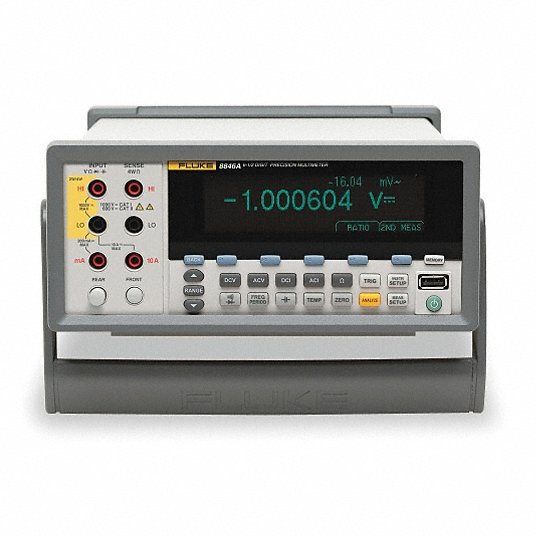
\includegraphics[scale=.25]{images/dmm_benchtop.jpeg}
					\tiny{Image: Fluke Multimeter}	 
					\vspace{50mm}

					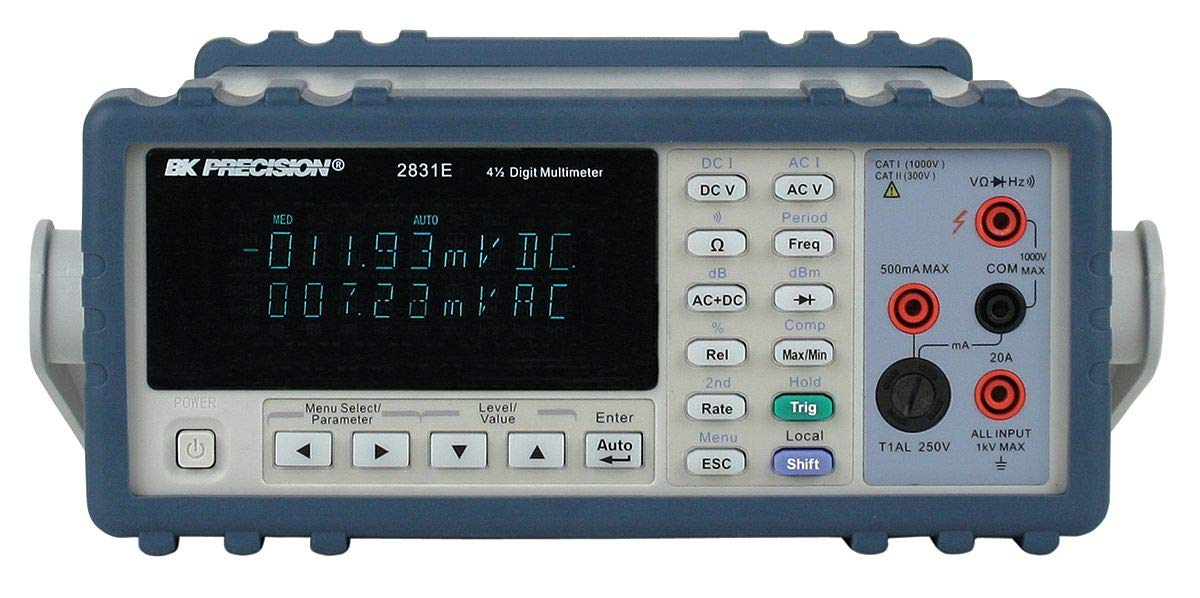
\includegraphics[scale=.13]{images/bk_2831e.jpg}
					\vspace{10mm}
					\tiny{Image: Bk Precision Multimeter }	
					\vspace{10mm}

				\end{multicols}	

			\end{frame}

			\begin{frame}
				\frametitle{\sectionIsubsectionIItitle}
				Handheld Multimeter

				\begin{multicols}{3}
					 
					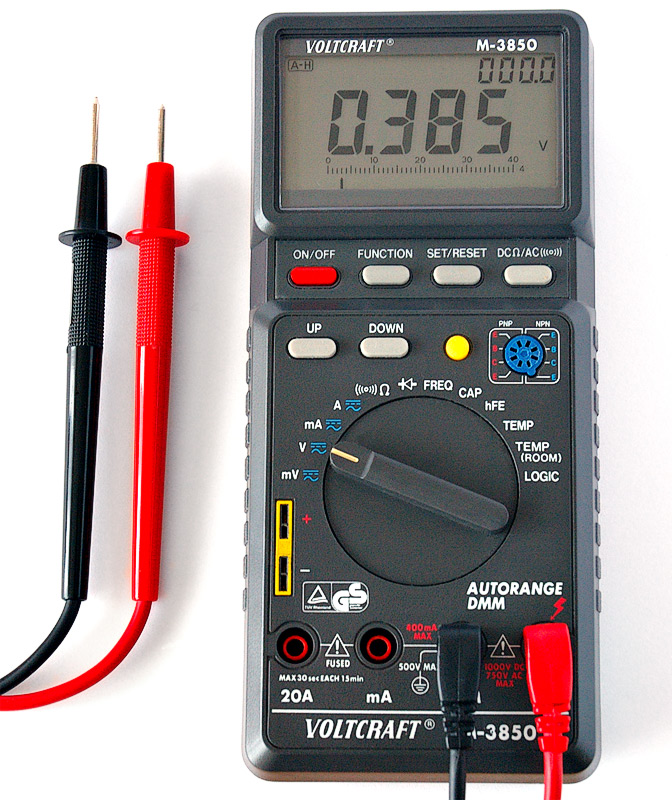
\includegraphics[scale=.15]{images/Digital_Multimeter_Aka.jpg}
					\tiny{Image: \href{https://commons.wikimedia.org/wiki/File:Digital_Multimeter_Aka.jpg}{Digital Multimeter - Wikimedia Commons}}

					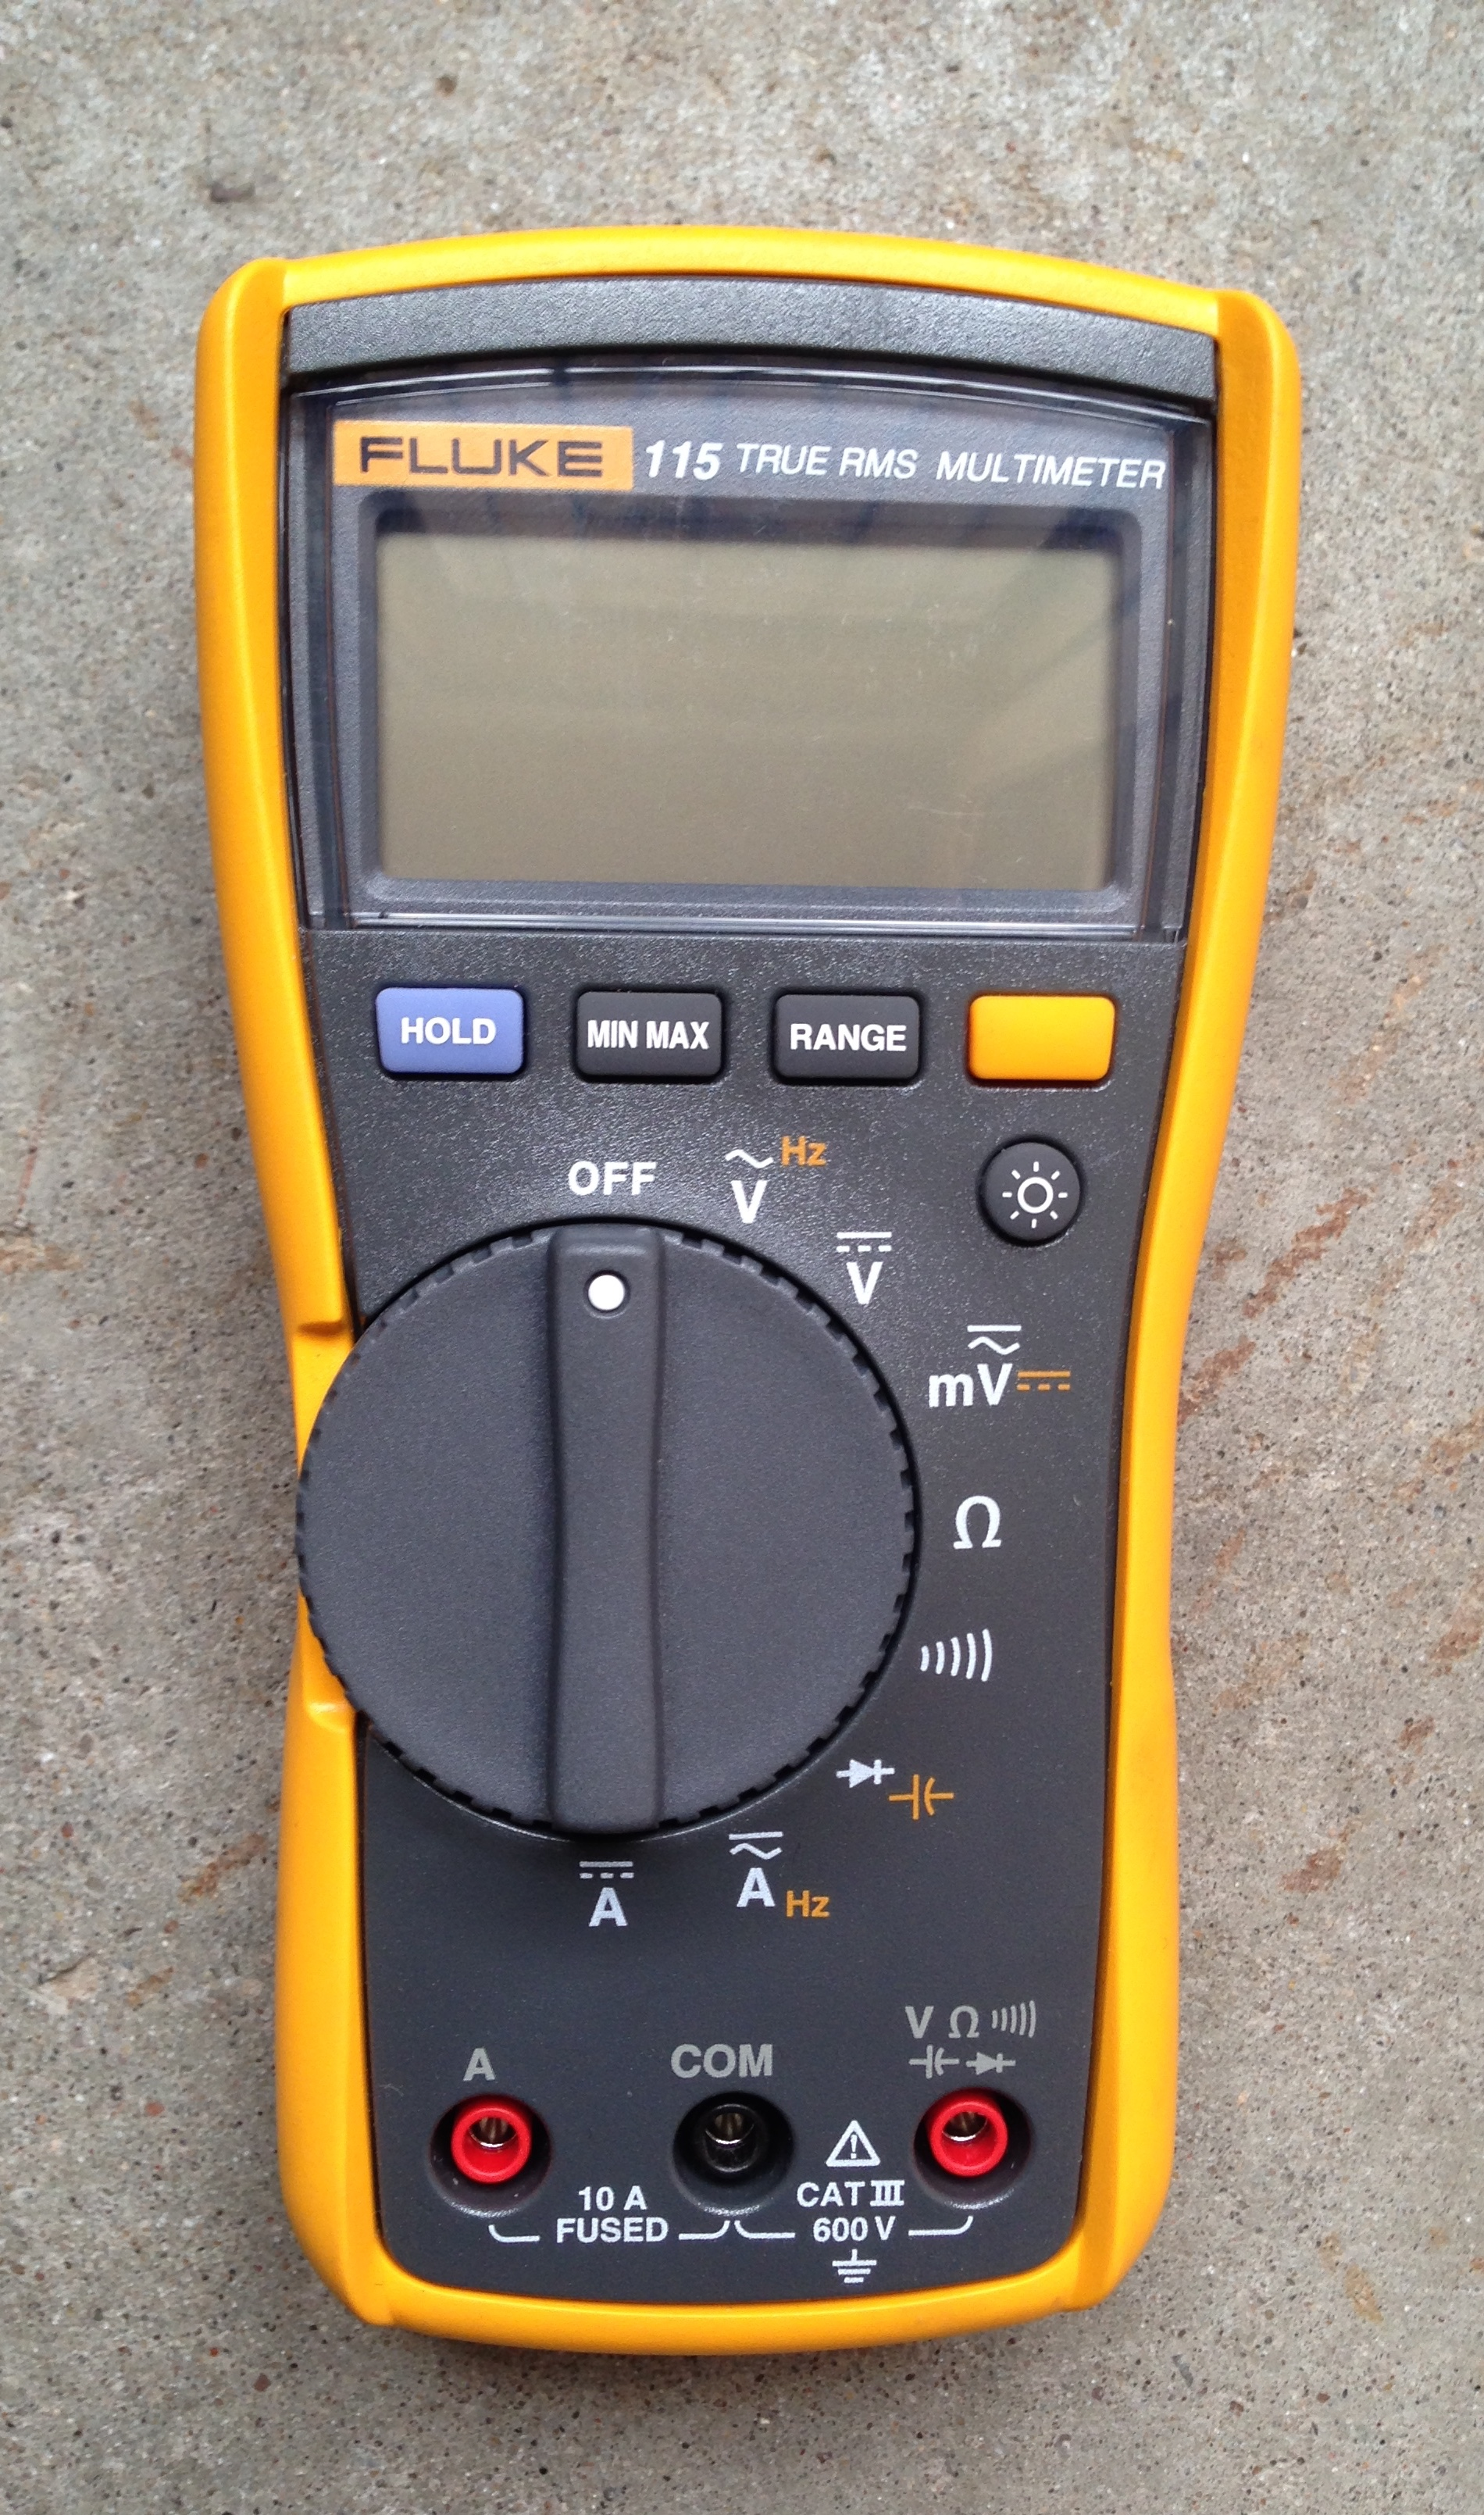
\includegraphics[scale=0.04]{images/Fluke_115_multimeter.jpeg}
					\tiny{Image:\href{https://commons.wikimedia.org/wiki/File:Fluke_115_multimeter.jpg}{Fluke 115 - Wikimedia Commons}}	
					
					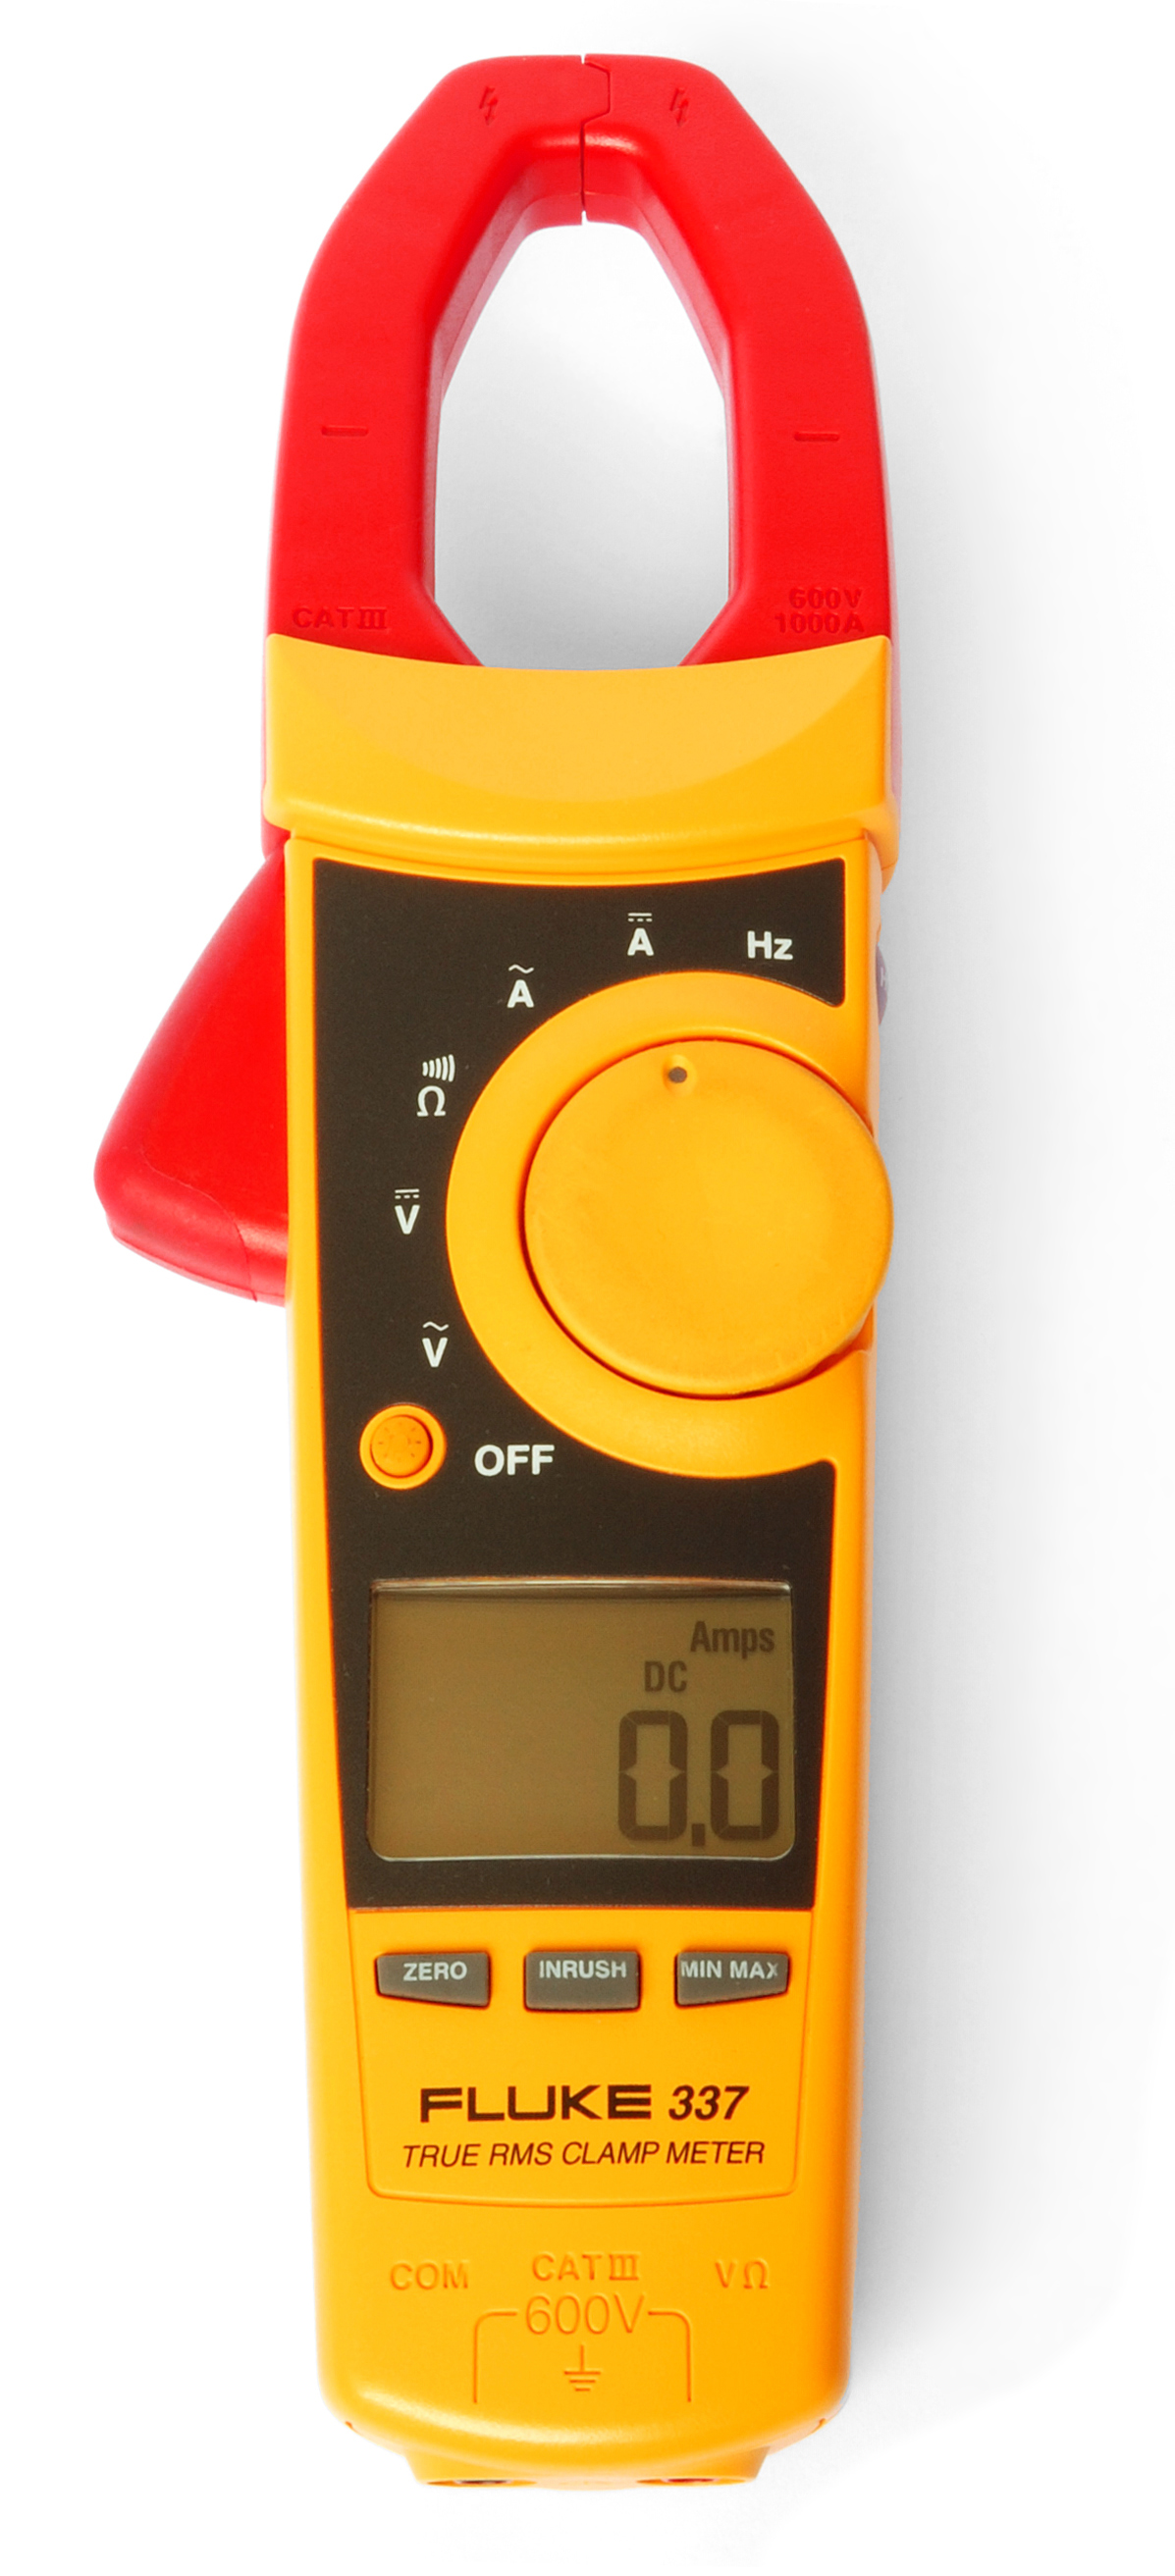
\includegraphics[scale=.20]{images/Clampmeter_Fluke_337}
					\tiny{Image: \href{https://commons.wikimedia.org/wiki/File:Clampmeter_Fluke_337.jpg}{Clampmeter 337 - Wikimedia Commons}}

				\end{multicols}	


			\end{frame}


		% section I subsection III
		\subsection{\sectionIsubsectionIIItitle}\label{sectionIsubsectionIII}
			\begin{frame} 
				\frametitle{\sectionIsubsectionIIItitle}
				\underline{{\bf \large Voltage}} \vspace{10mm}\\ 

				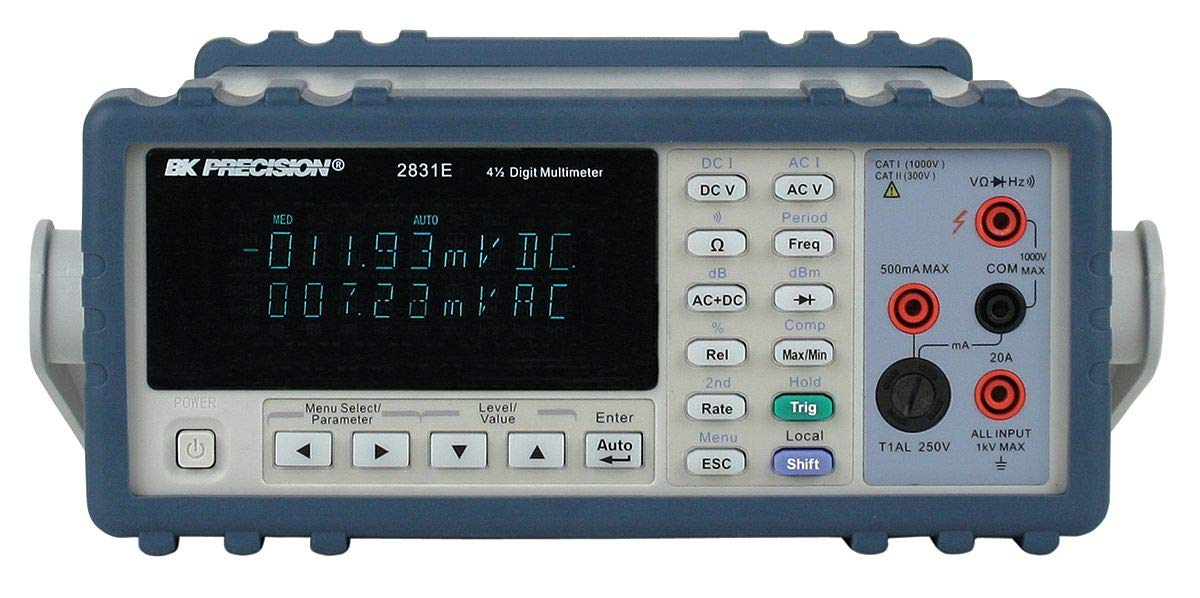
\includegraphics[scale=.13]{images/bk_2831e.jpg}
				\vspace{10mm}
				\tiny{Image: Bk Precision Multimeter }

				\textbf{ \href{https://www.fluke.com/en-us/learn/best-practices/test-tools-basics/digital-multimeters/how-to-measure-dc-voltage-with-a-digital-multimeter}{Read about measuring DC voltage} }

				\textbf{or \href{https://www.fluke.com/en-us/learn/best-practices/test-tools-basics/digital-multimeters/how-to-measure-ac-voltage-with-a-digital-multimeter}{ AC voltage} }

			\end{frame}	

			\begin{frame} 
				\frametitle{\sectionIsubsectionIIItitle}
				\underline{{\bf Current}} \vspace{10mm}\\  
 
				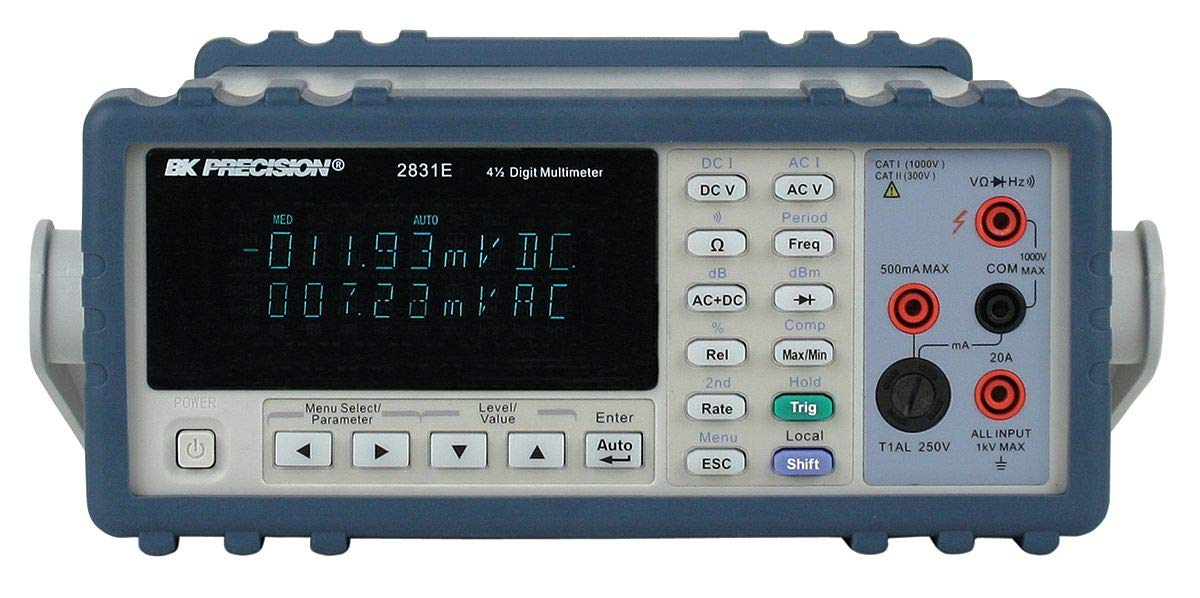
\includegraphics[scale=.13]{images/bk_2831e.jpg}
				\vspace{10mm}
				\tiny{Image: Bk Precision Multimeter }

				\textbf{ \href{https://www.fluke.com/en-us/learn/best-practices/test-tools-basics/digital-multimeters/how-to-measure-current-with-a-digital-multimeter-plus-clamp-accessory}{Read about measuring current (with clamp)} }

			\end{frame}	

		% section I subsection IV
		\subsection{\sectionIsubsectionIVtitle}\label{sectionIsubsectionIV}	

			\begin{frame}
				\frametitle{\sectionIsubsectionIVtitle}
				\underline{{\bf \large Resistance}} \vspace{10mm}\\ 

				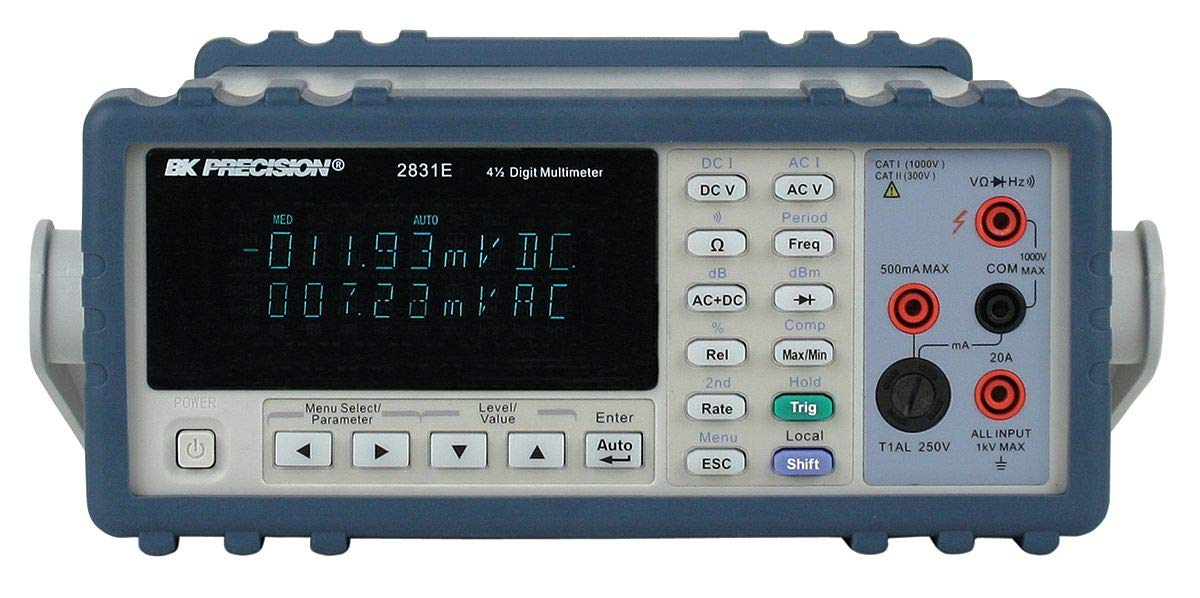
\includegraphics[scale=.13]{images/bk_2831e.jpg}
				\vspace{10mm}
				\tiny{Image: Bk Precision Multimeter }

				\textbf{ \href{https://www.fluke.com/en-us/learn/best-practices/test-tools-basics/digital-multimeters/how-to-measure-resistance}{Read about measuring resistance} }

			\end{frame}

			\begin{frame}
				\frametitle{\sectionIsubsectionIVtitle}
				\underline{{\bf \large Continuity}} \vspace{10mm}\\ 

				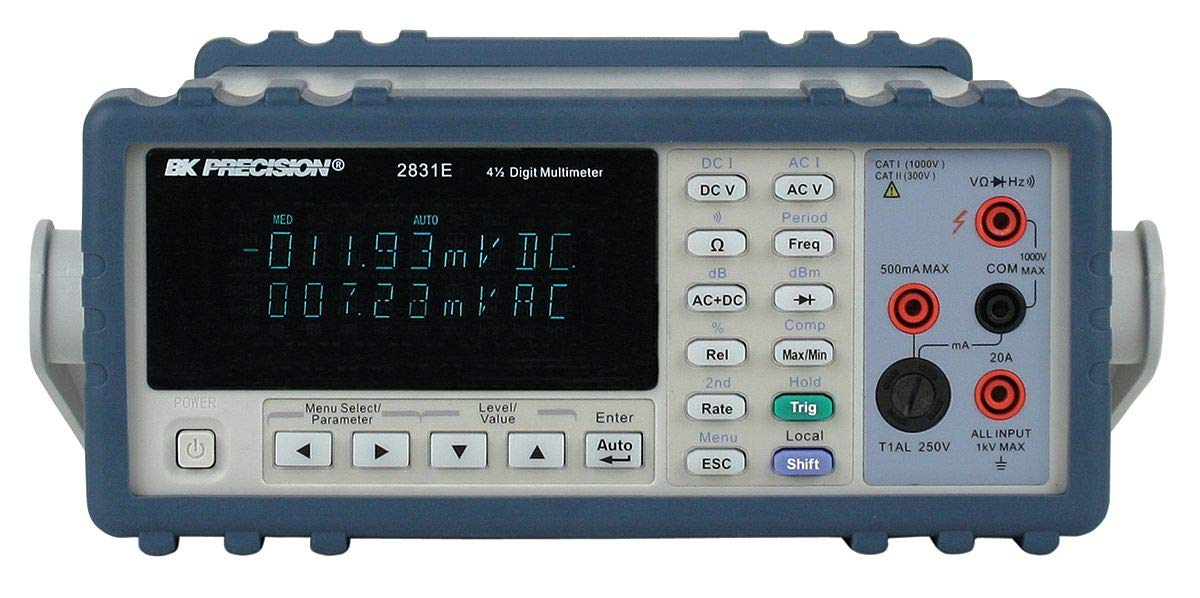
\includegraphics[scale=.13]{images/bk_2831e.jpg}
				\vspace{10mm}
				\tiny{Image: Bk Precision Multimeter }

				\textbf{ \href{https://www.fluke.com/en-us/learn/best-practices/test-tools-basics/digital-multimeters/how-to-test-for-continuity-with-a-digital-multimeter}{Read about measuring continuity} } 
	 
			\end{frame}

	
	% Section II
	\section{\sectionIItitle}\label{sectionII}

		% section II Outline
		\begin{frame}
			\large \textbf{Topic 2 - \sectionIItitle} \vspace{3mm}\\

			\begin{itemize}
				\item \hyperlink{sectionIIsubsectionI}{\sectionIIsubsectionItitle} \vspc %  section II subsection I
				\item \hyperlink{sectionIIsubsectionII}{\sectionIIsubsectionIItitle} \vspc % section II subsection II
				\item \hyperlink{sectionIIsubsectionIII}{\sectionIIsubsectionIIItitle} \vspc % section II subsection III
				\item \hyperlink{sectionIIsubsectionIV}{\sectionIIsubsectionIVtitle} \vspc % section II subsection IV
			\end{itemize}
		\end{frame}

		% section II subsection I
		\subsection{\sectionIIsubsectionItitle}\label{sectionIIsubsectionI}

			\begin{frame}[label=sectionIIsubsectionI]
				\frametitle{\sectionIIsubsectionItitle}

				Engineering is an integrated field...

			\end{frame}

		% section II subsection II
		\subsection{\sectionIIsubsectionIItitle}\label{sectionIIsubsectionII}

			\begin{frame}
				\frametitle{\sectionIIsubsectionIItitle}

				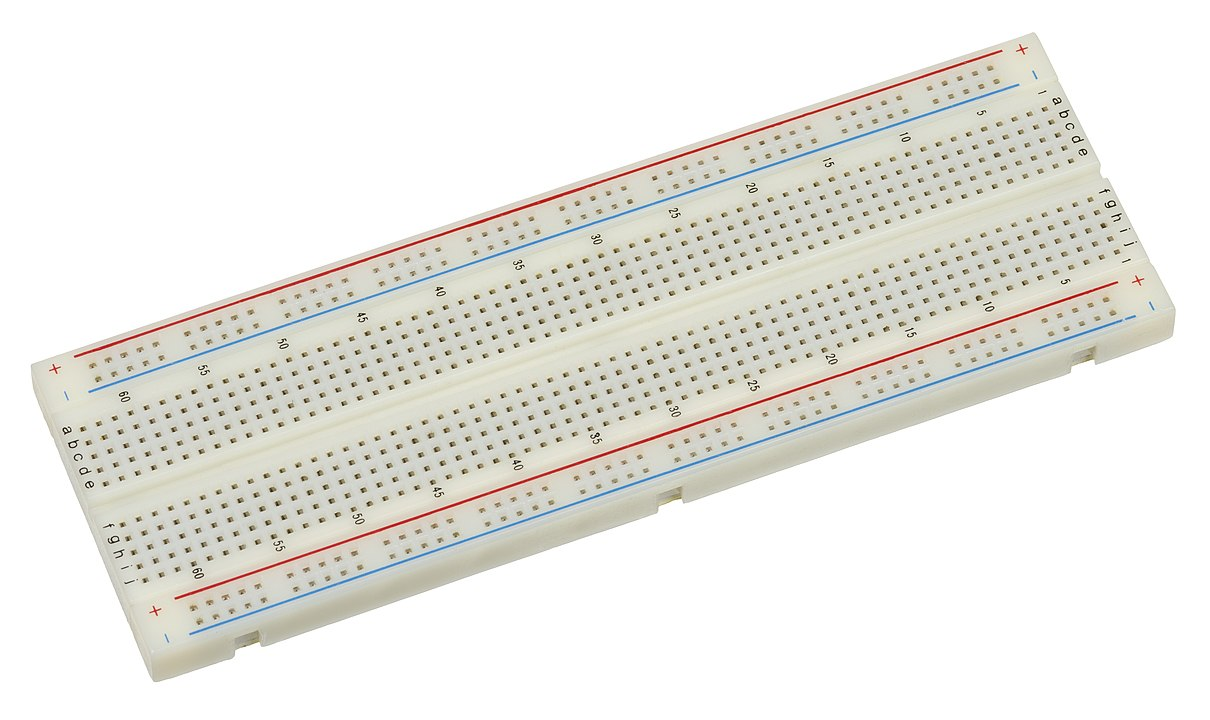
\includegraphics[scale=.125]{images/breadboard_large.jpg} 	
				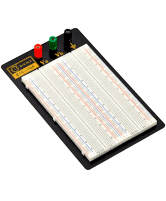
\includegraphics[scale=.65]{images/breadboard_wplugs.png} 
		

			\end{frame}

			\begin{frame}
				\frametitle{\sectionIIsubsectionIItitle}

				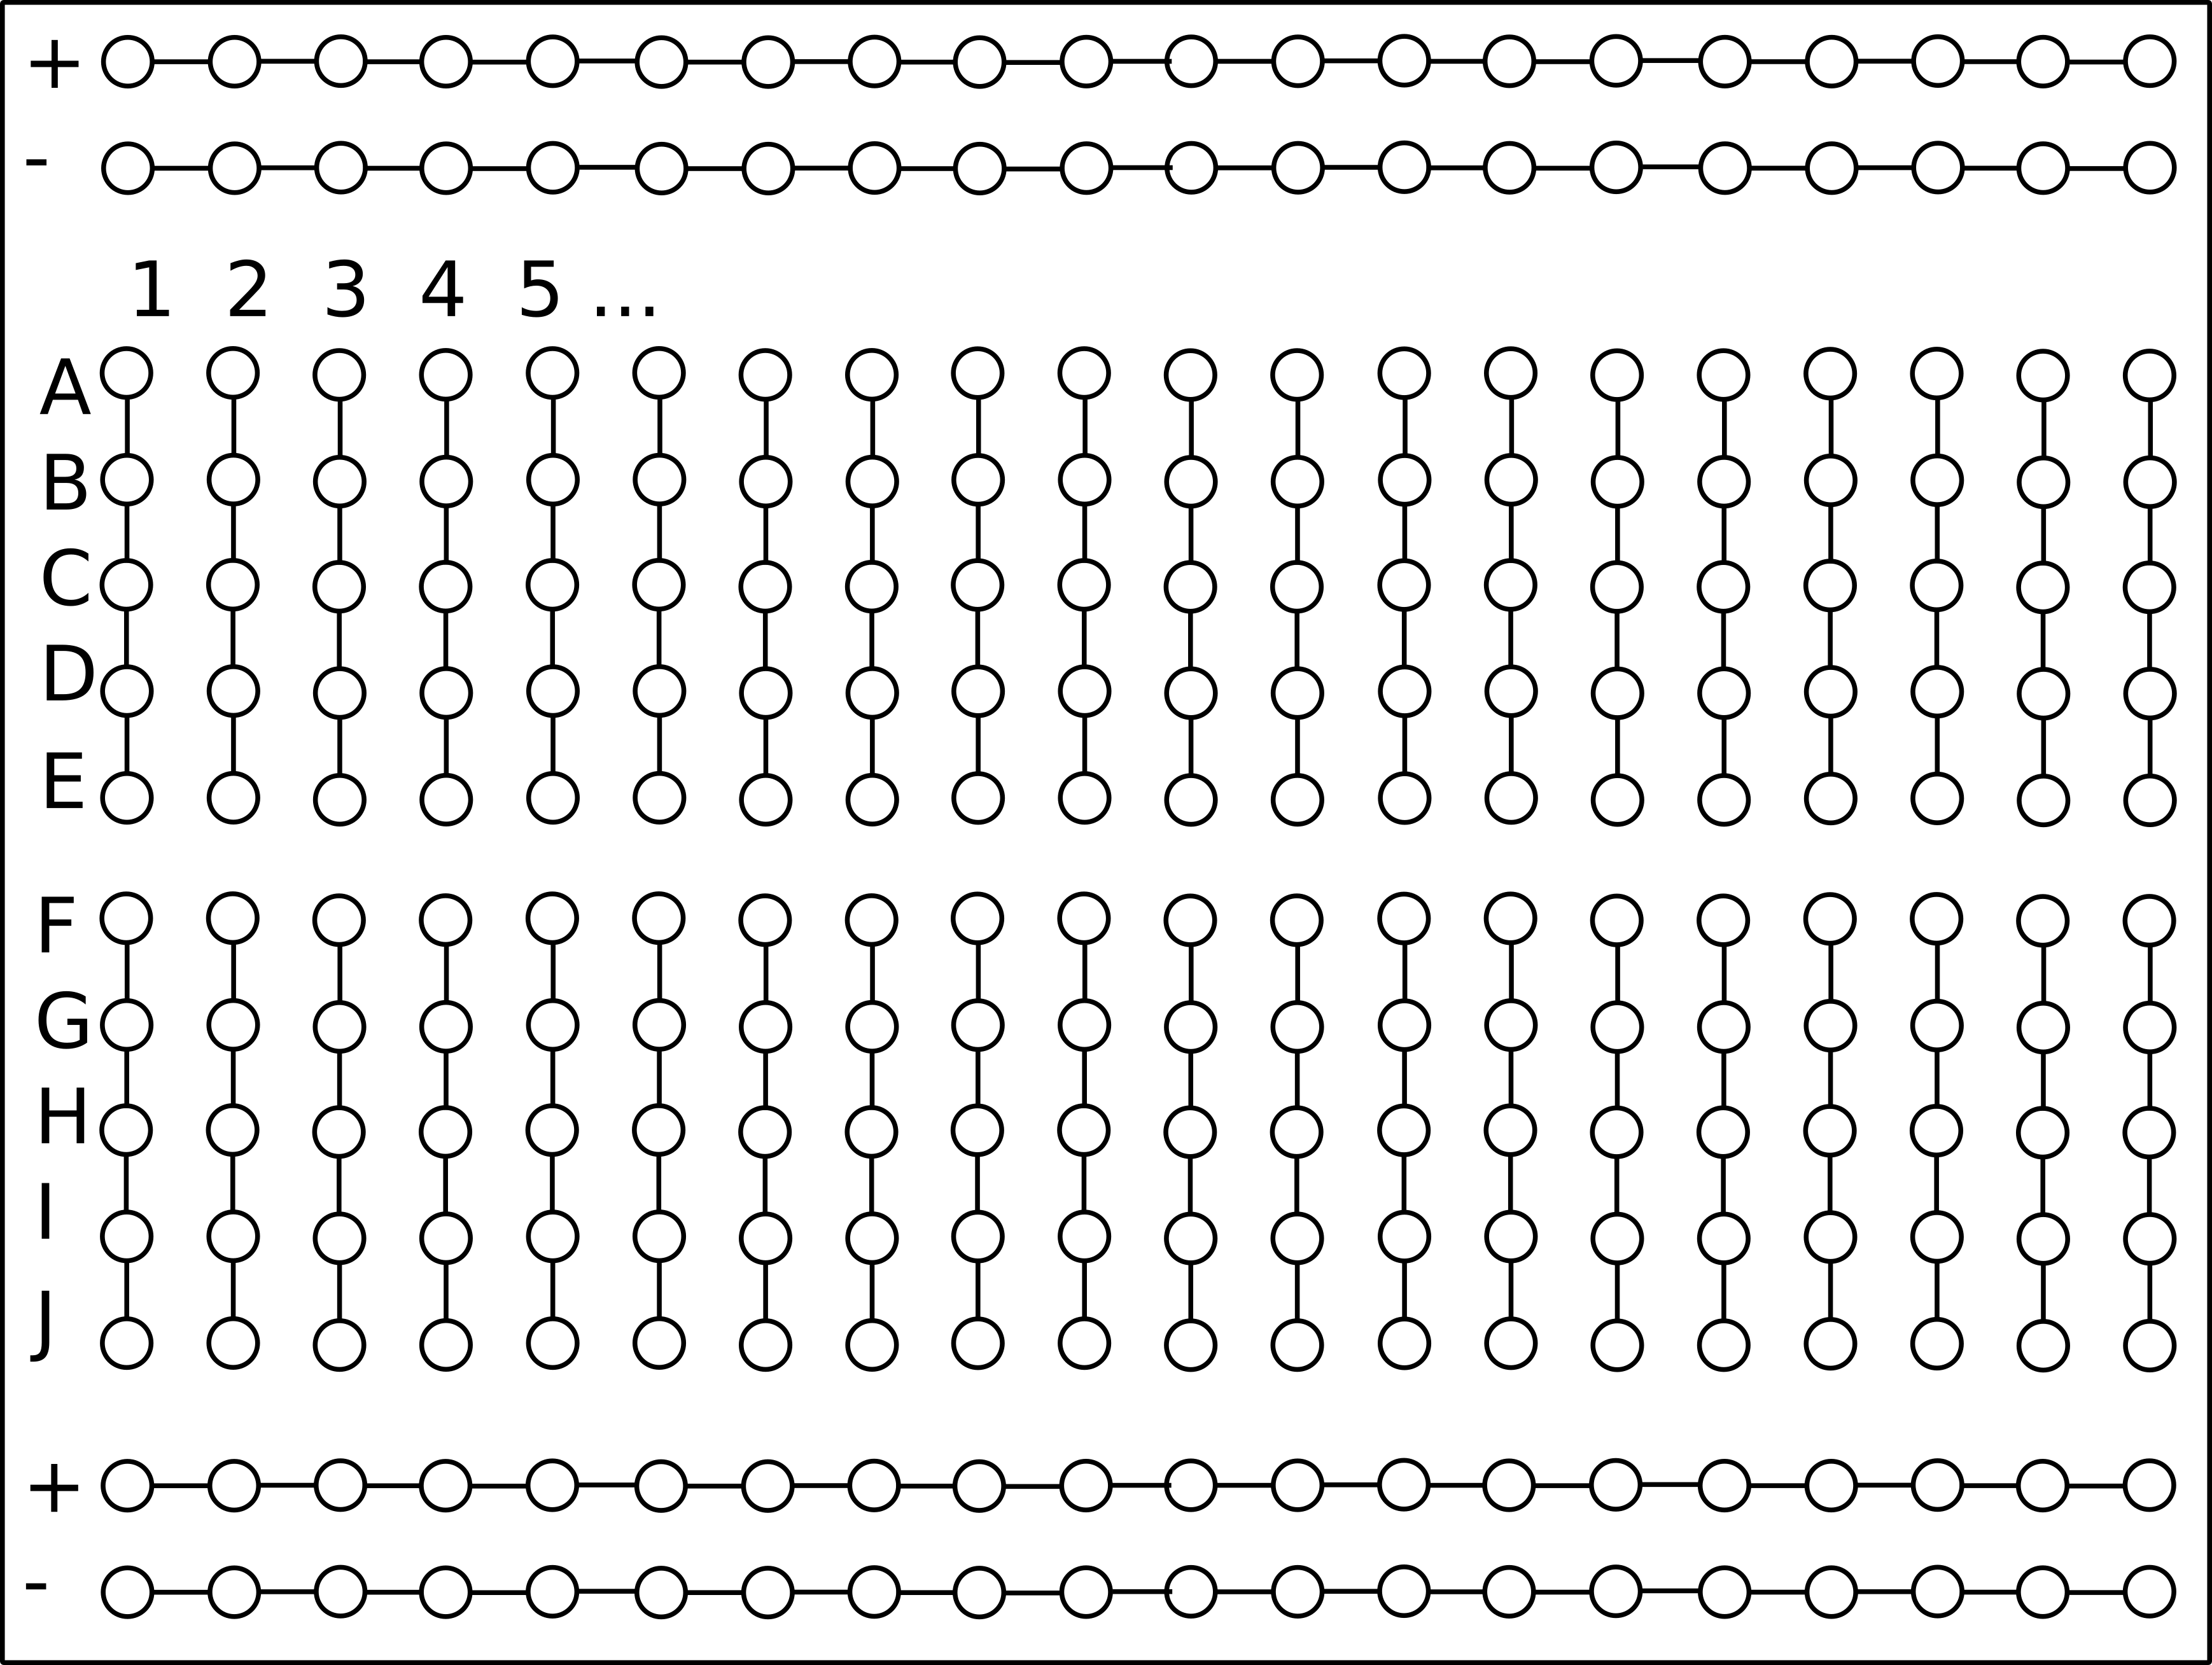
\includegraphics[scale=.080]{images/breadboard_template.png}
		

			\end{frame}

			\begin{frame}
				\frametitle{\sectionIIsubsectionIItitle}

				Example 1:

				Question: Why is the breadboard separated into sections? 
				(note: this image shows 4 - top,bottom,top,bottom) 

				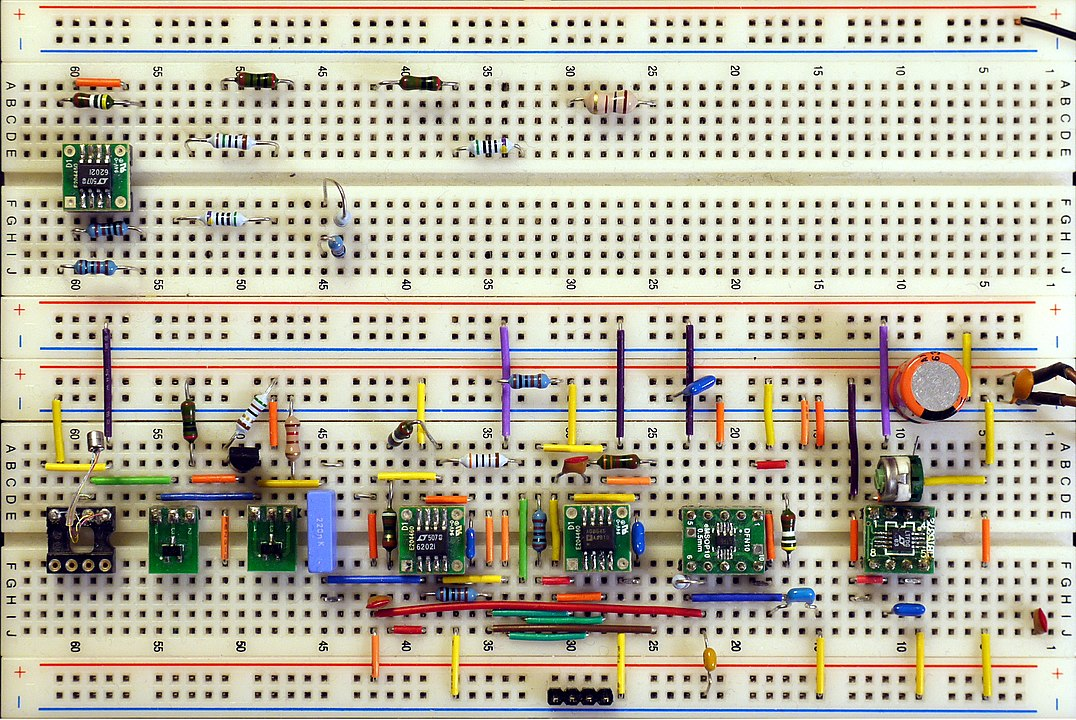
\includegraphics[scale=.20]{images/breadboard_wcircuit.jpg}

			\end{frame}

			\begin{frame}
				\frametitle{\sectionIIsubsectionIItitle}

				Example 2:

	  			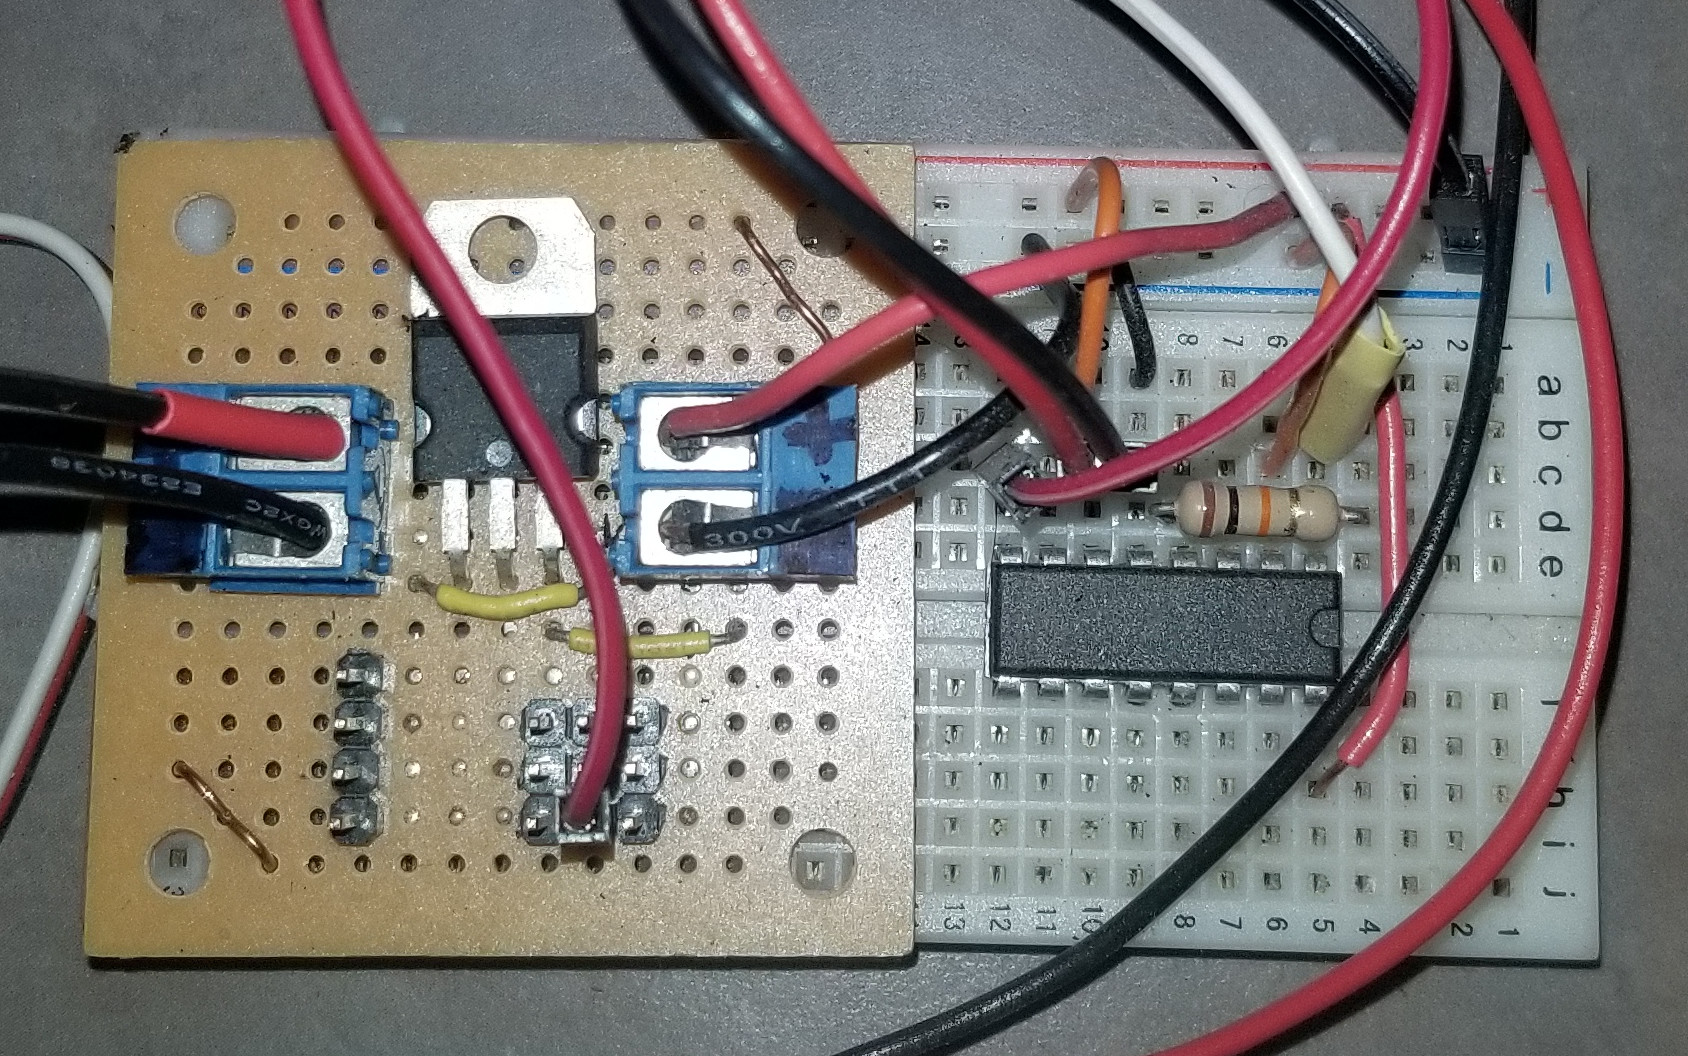
\includegraphics[scale=.1]{images/breadboard_fan_hbridge_cropped.jpg} 

			\end{frame}

			\begin{frame}
				\frametitle{\sectionIIsubsectionIItitle}

				Example 3:

	  			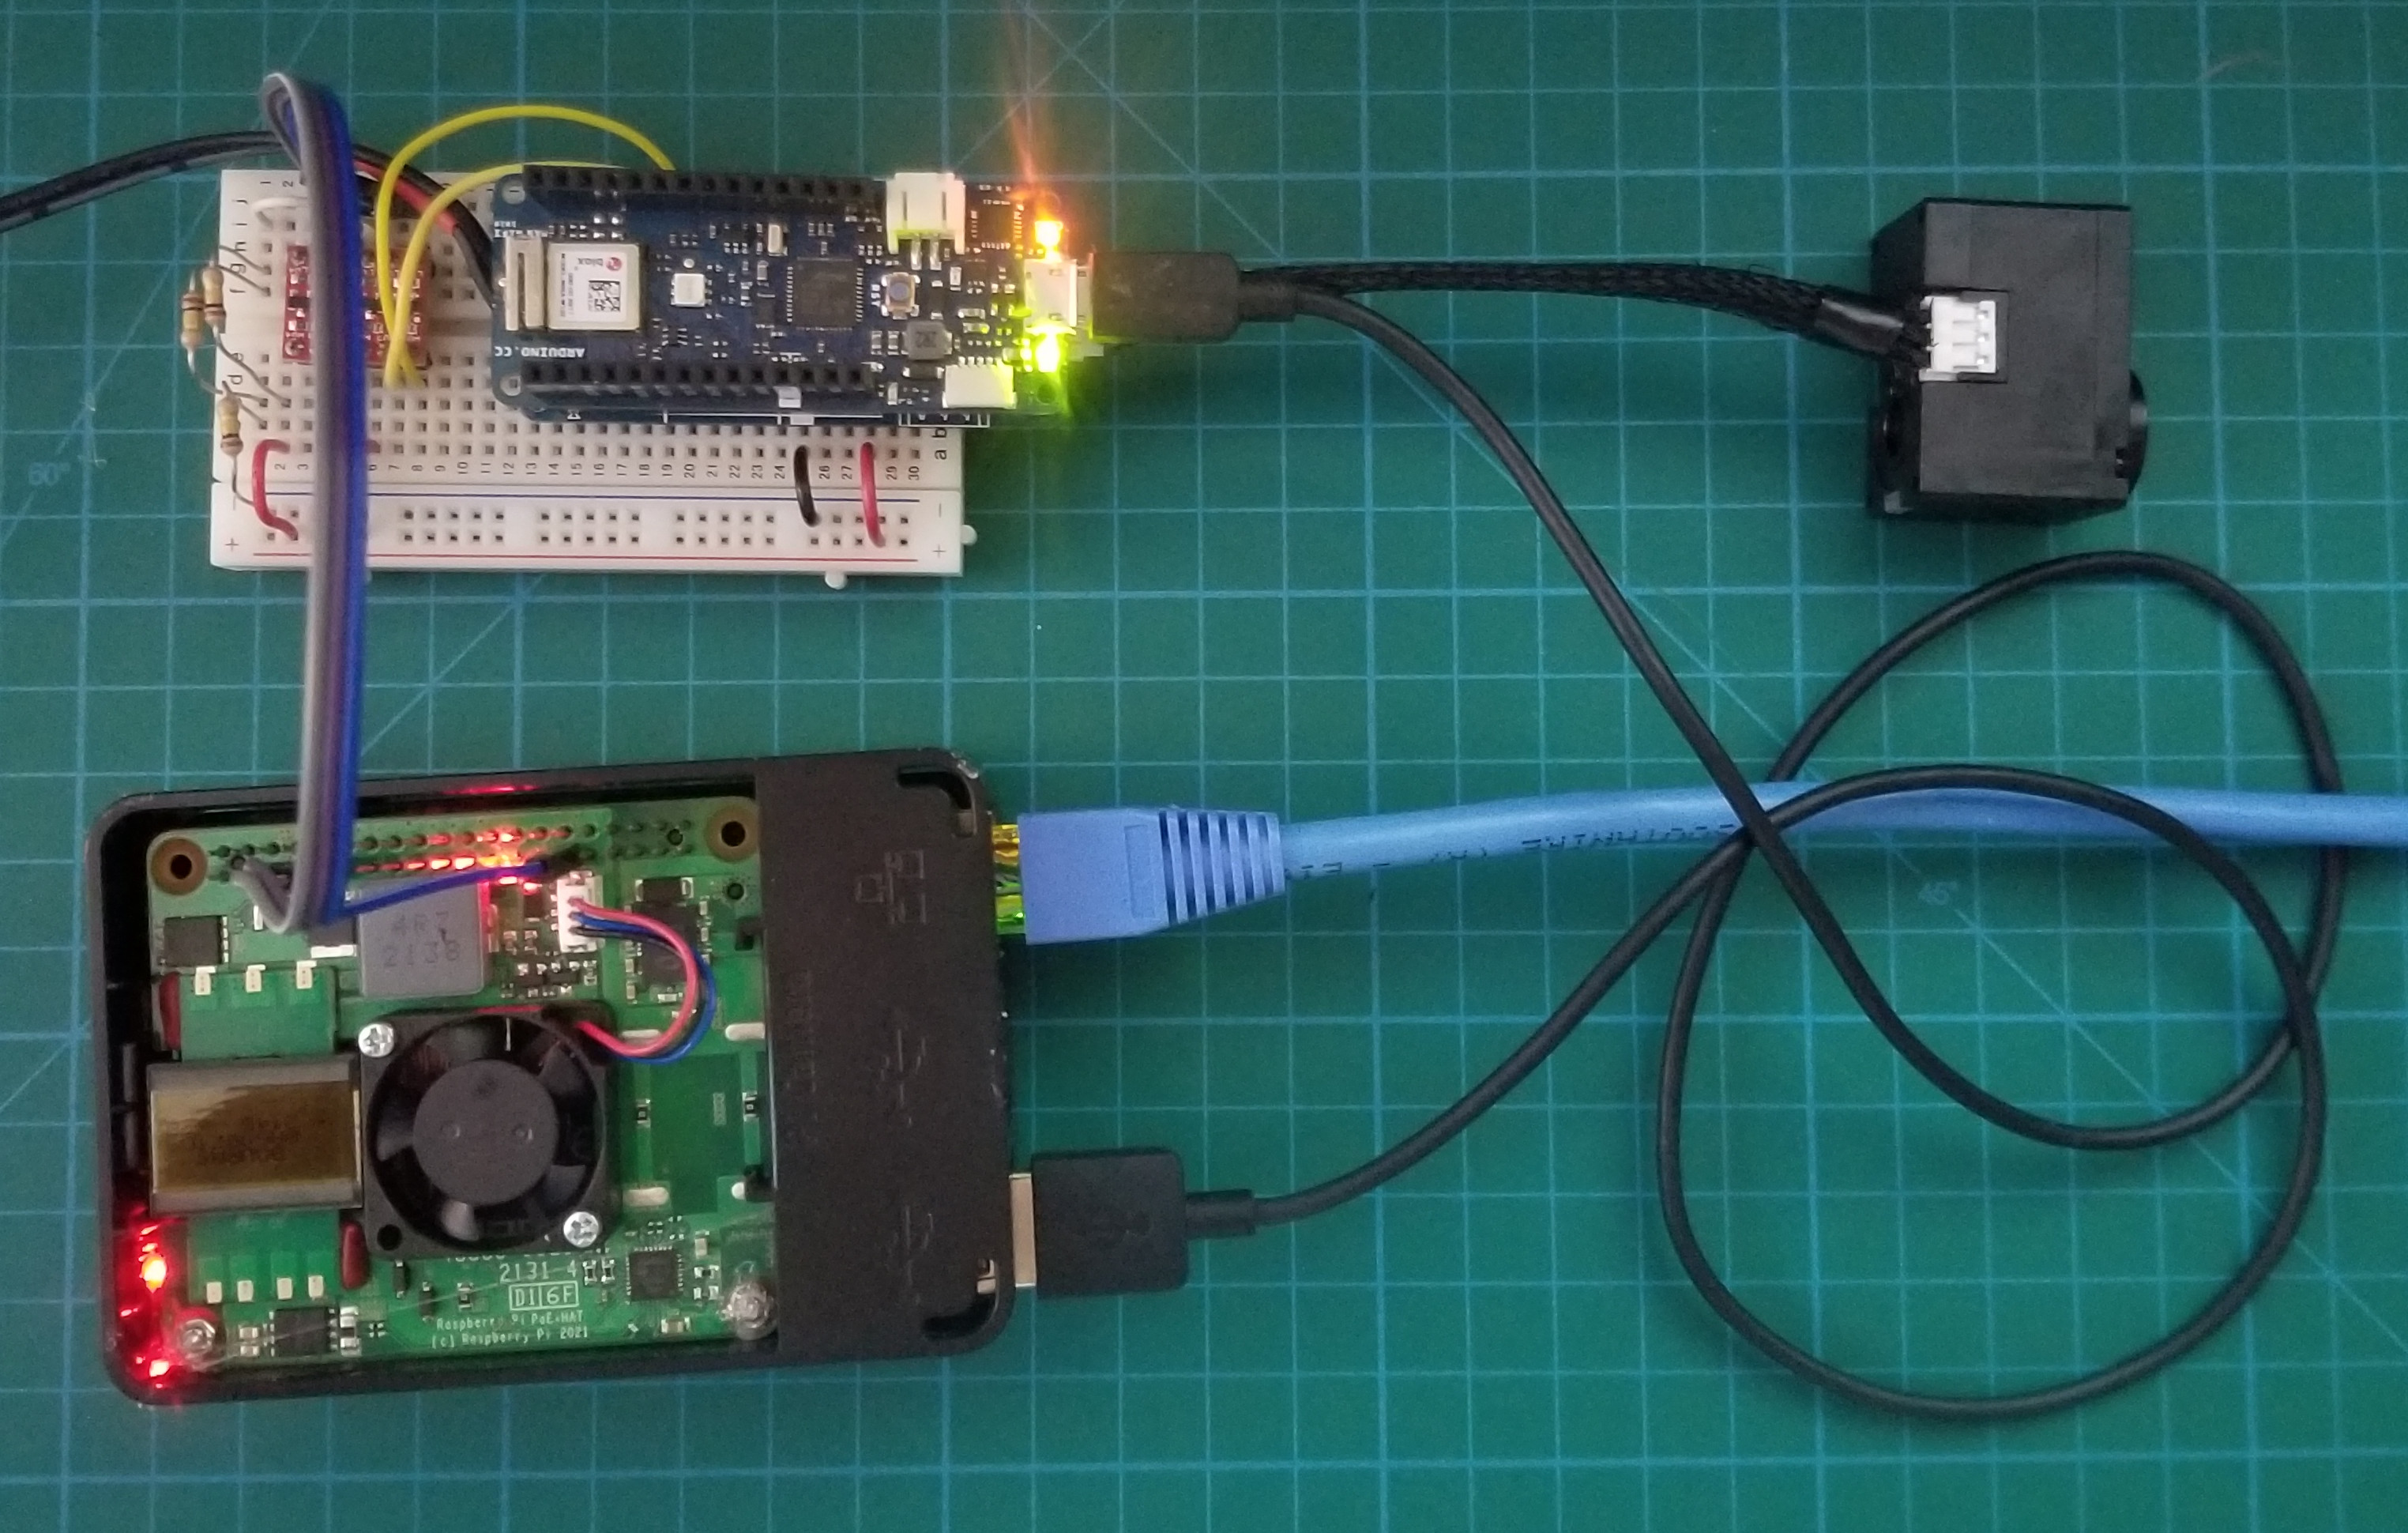
\includegraphics[scale=.04]{images/breadboard_arduino_rpi_cropped.jpg} 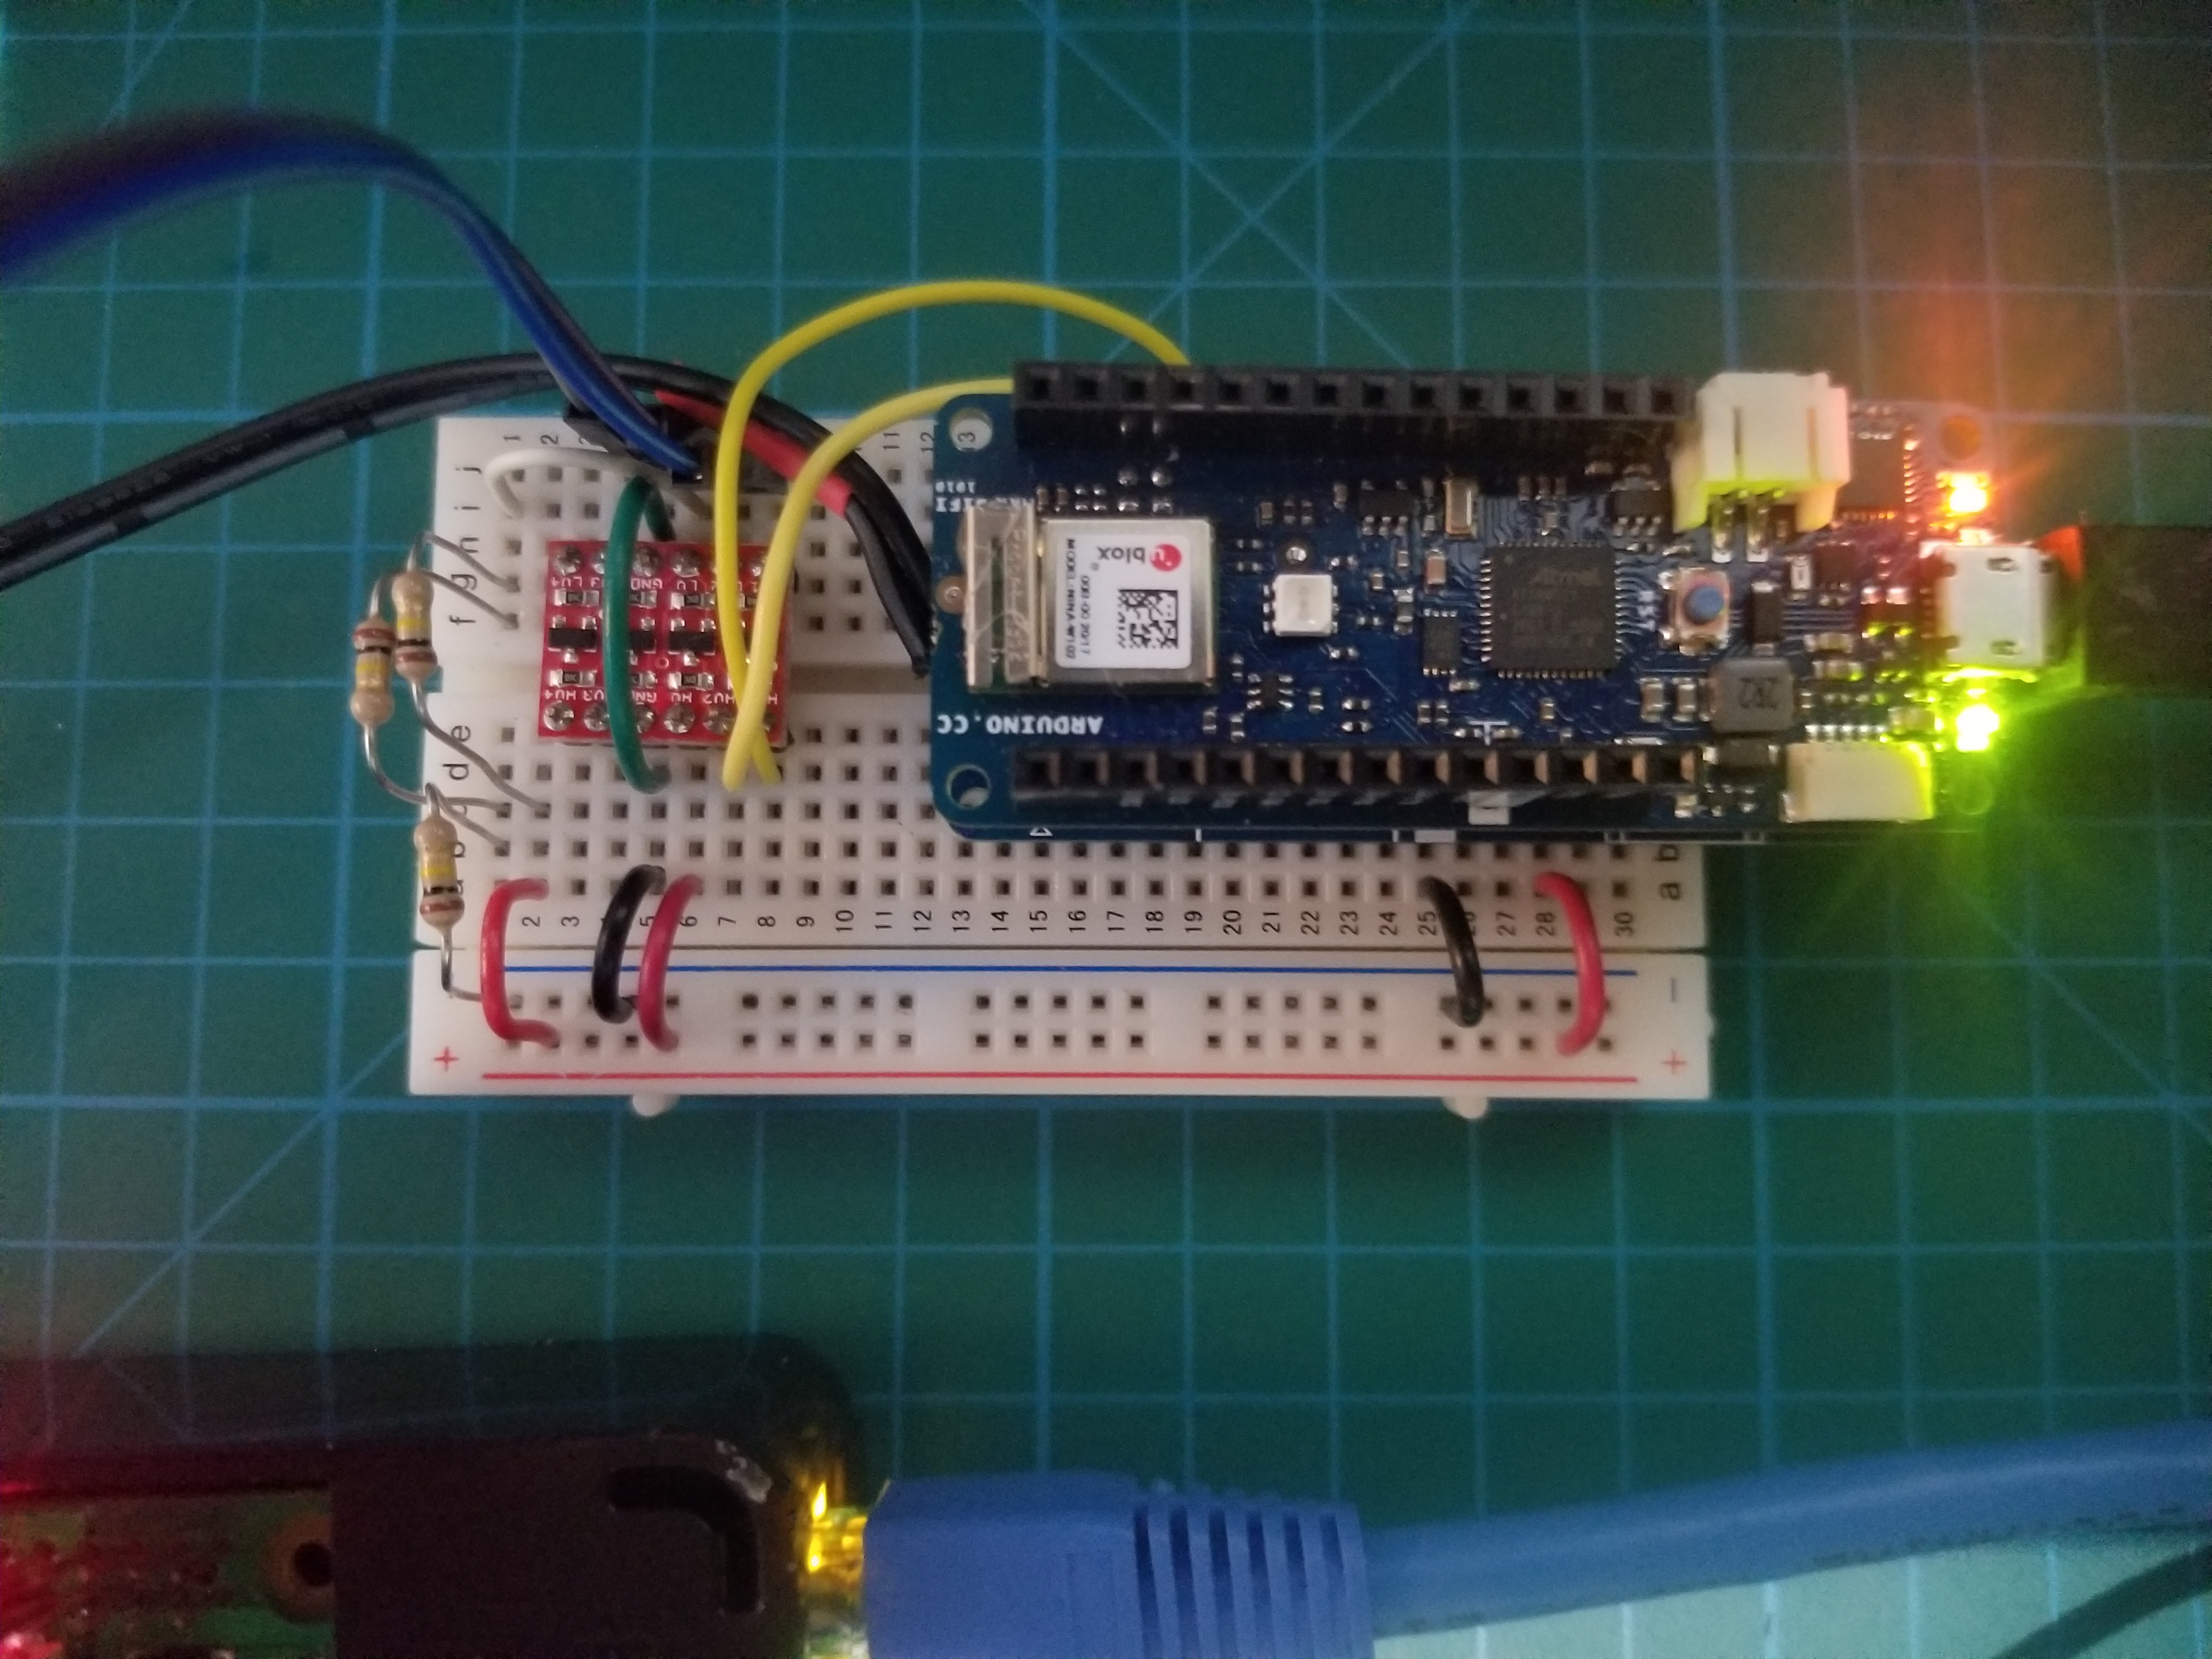
\includegraphics[scale=.0275]{images/breadboard_arduino_serial.jpg}
	  			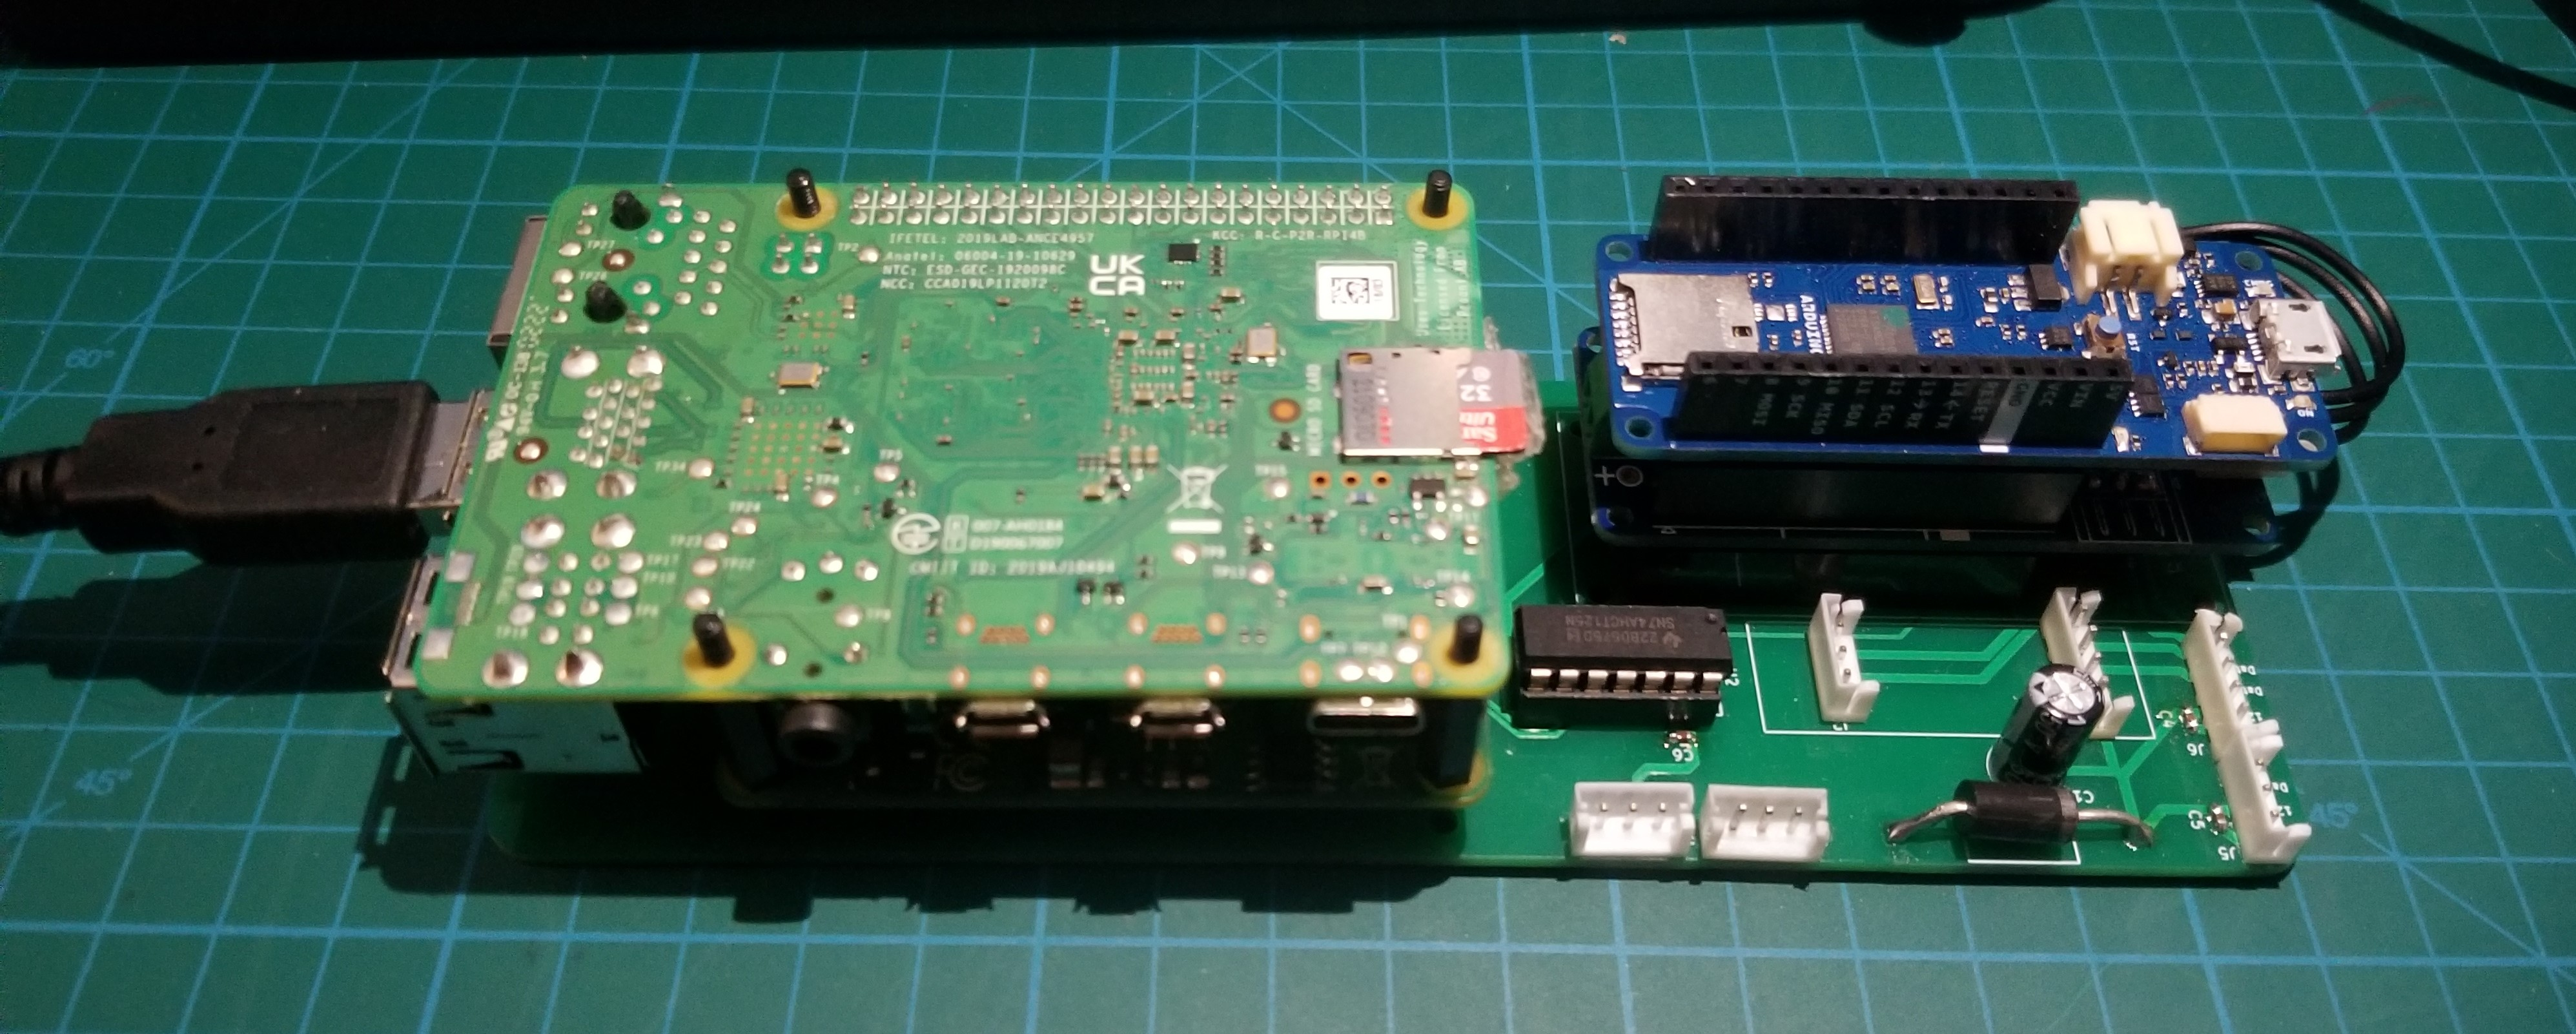
\includegraphics[scale=0.05]{images/sbc_mcu_carrier_v1.jpg}

			\end{frame}

			\begin{frame}
				\frametitle{\sectionIIsubsectionIItitle}

				 \begin{multicols}{2}
					 \underline{Pros:}
					 
					 \underline{Cons:}
					 
				 \end{multicols}
				 \vspace{30mm}
				 
				 \underline{Common Mistakes:}
				 \vspace{10mm}
			
			\end{frame}



		% section II subsection III
		\subsection{\sectionIIsubsectionIIItitle}\label{sectionIIsubsectionIII}

			\begin{frame}
				\frametitle{\sectionIIsubsectionIIItitle}

				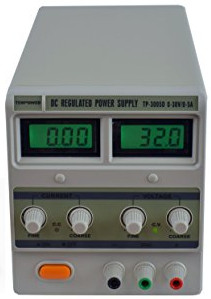
\includegraphics[scale=1.7]{images/lab_psu_cropped.jpg} 
				\hspace{5mm} 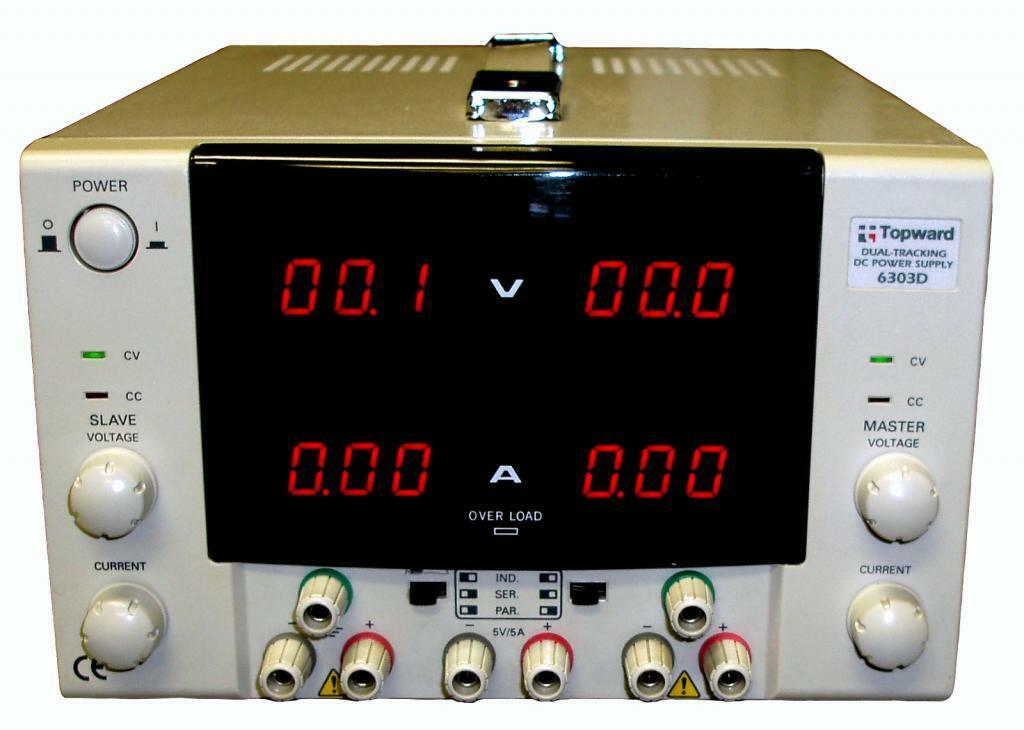
\includegraphics[scale=.17]{images/topward.jpg}

			\end{frame}

			\begin{frame}
				\frametitle{\sectionIIsubsectionIIItitle}

				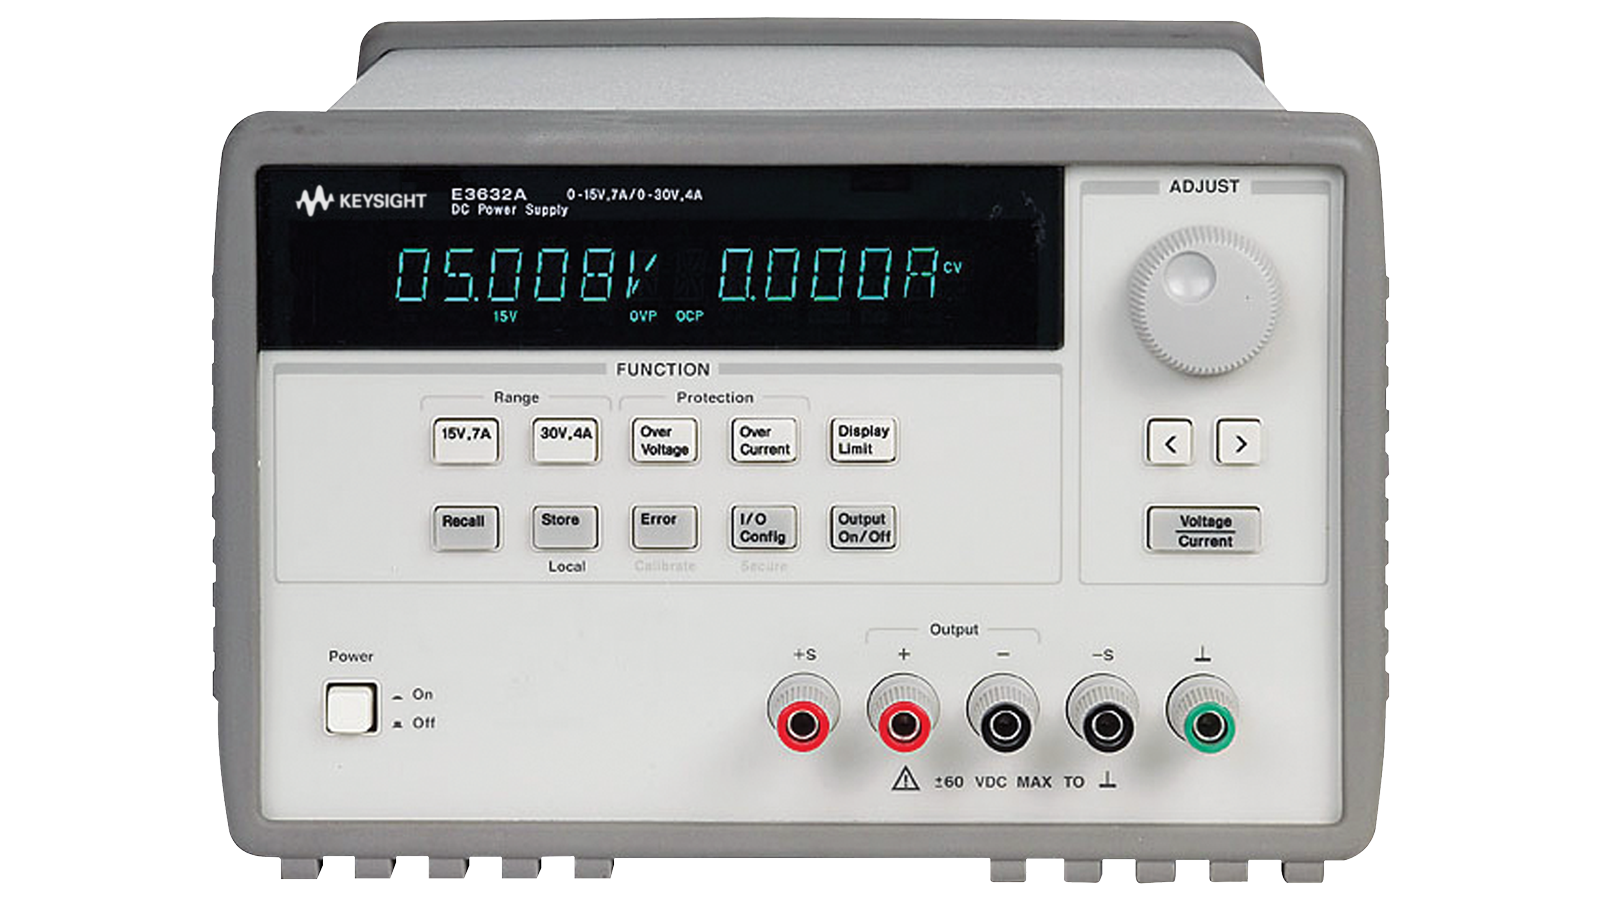
\includegraphics[scale=.15]{images/hp_psu.png} 

			\end{frame}

			\begin{frame}
			\frametitle{\sectionIIsubsectionIIItitle}

				\begin{itemize}

					\item - Equippment Saftey \vspccc
					\item - Damage \vspccc
					\item - Protection \vspccc

				\end{itemize}

			\end{frame}

		% section II subsection IV 
		\subsection{\sectionIIsubsectionIVtitle}\label{sectionIIsubsectionIV}

			\begin{frame}
				\frametitle{\sectionIIsubsectionIVtitle}

				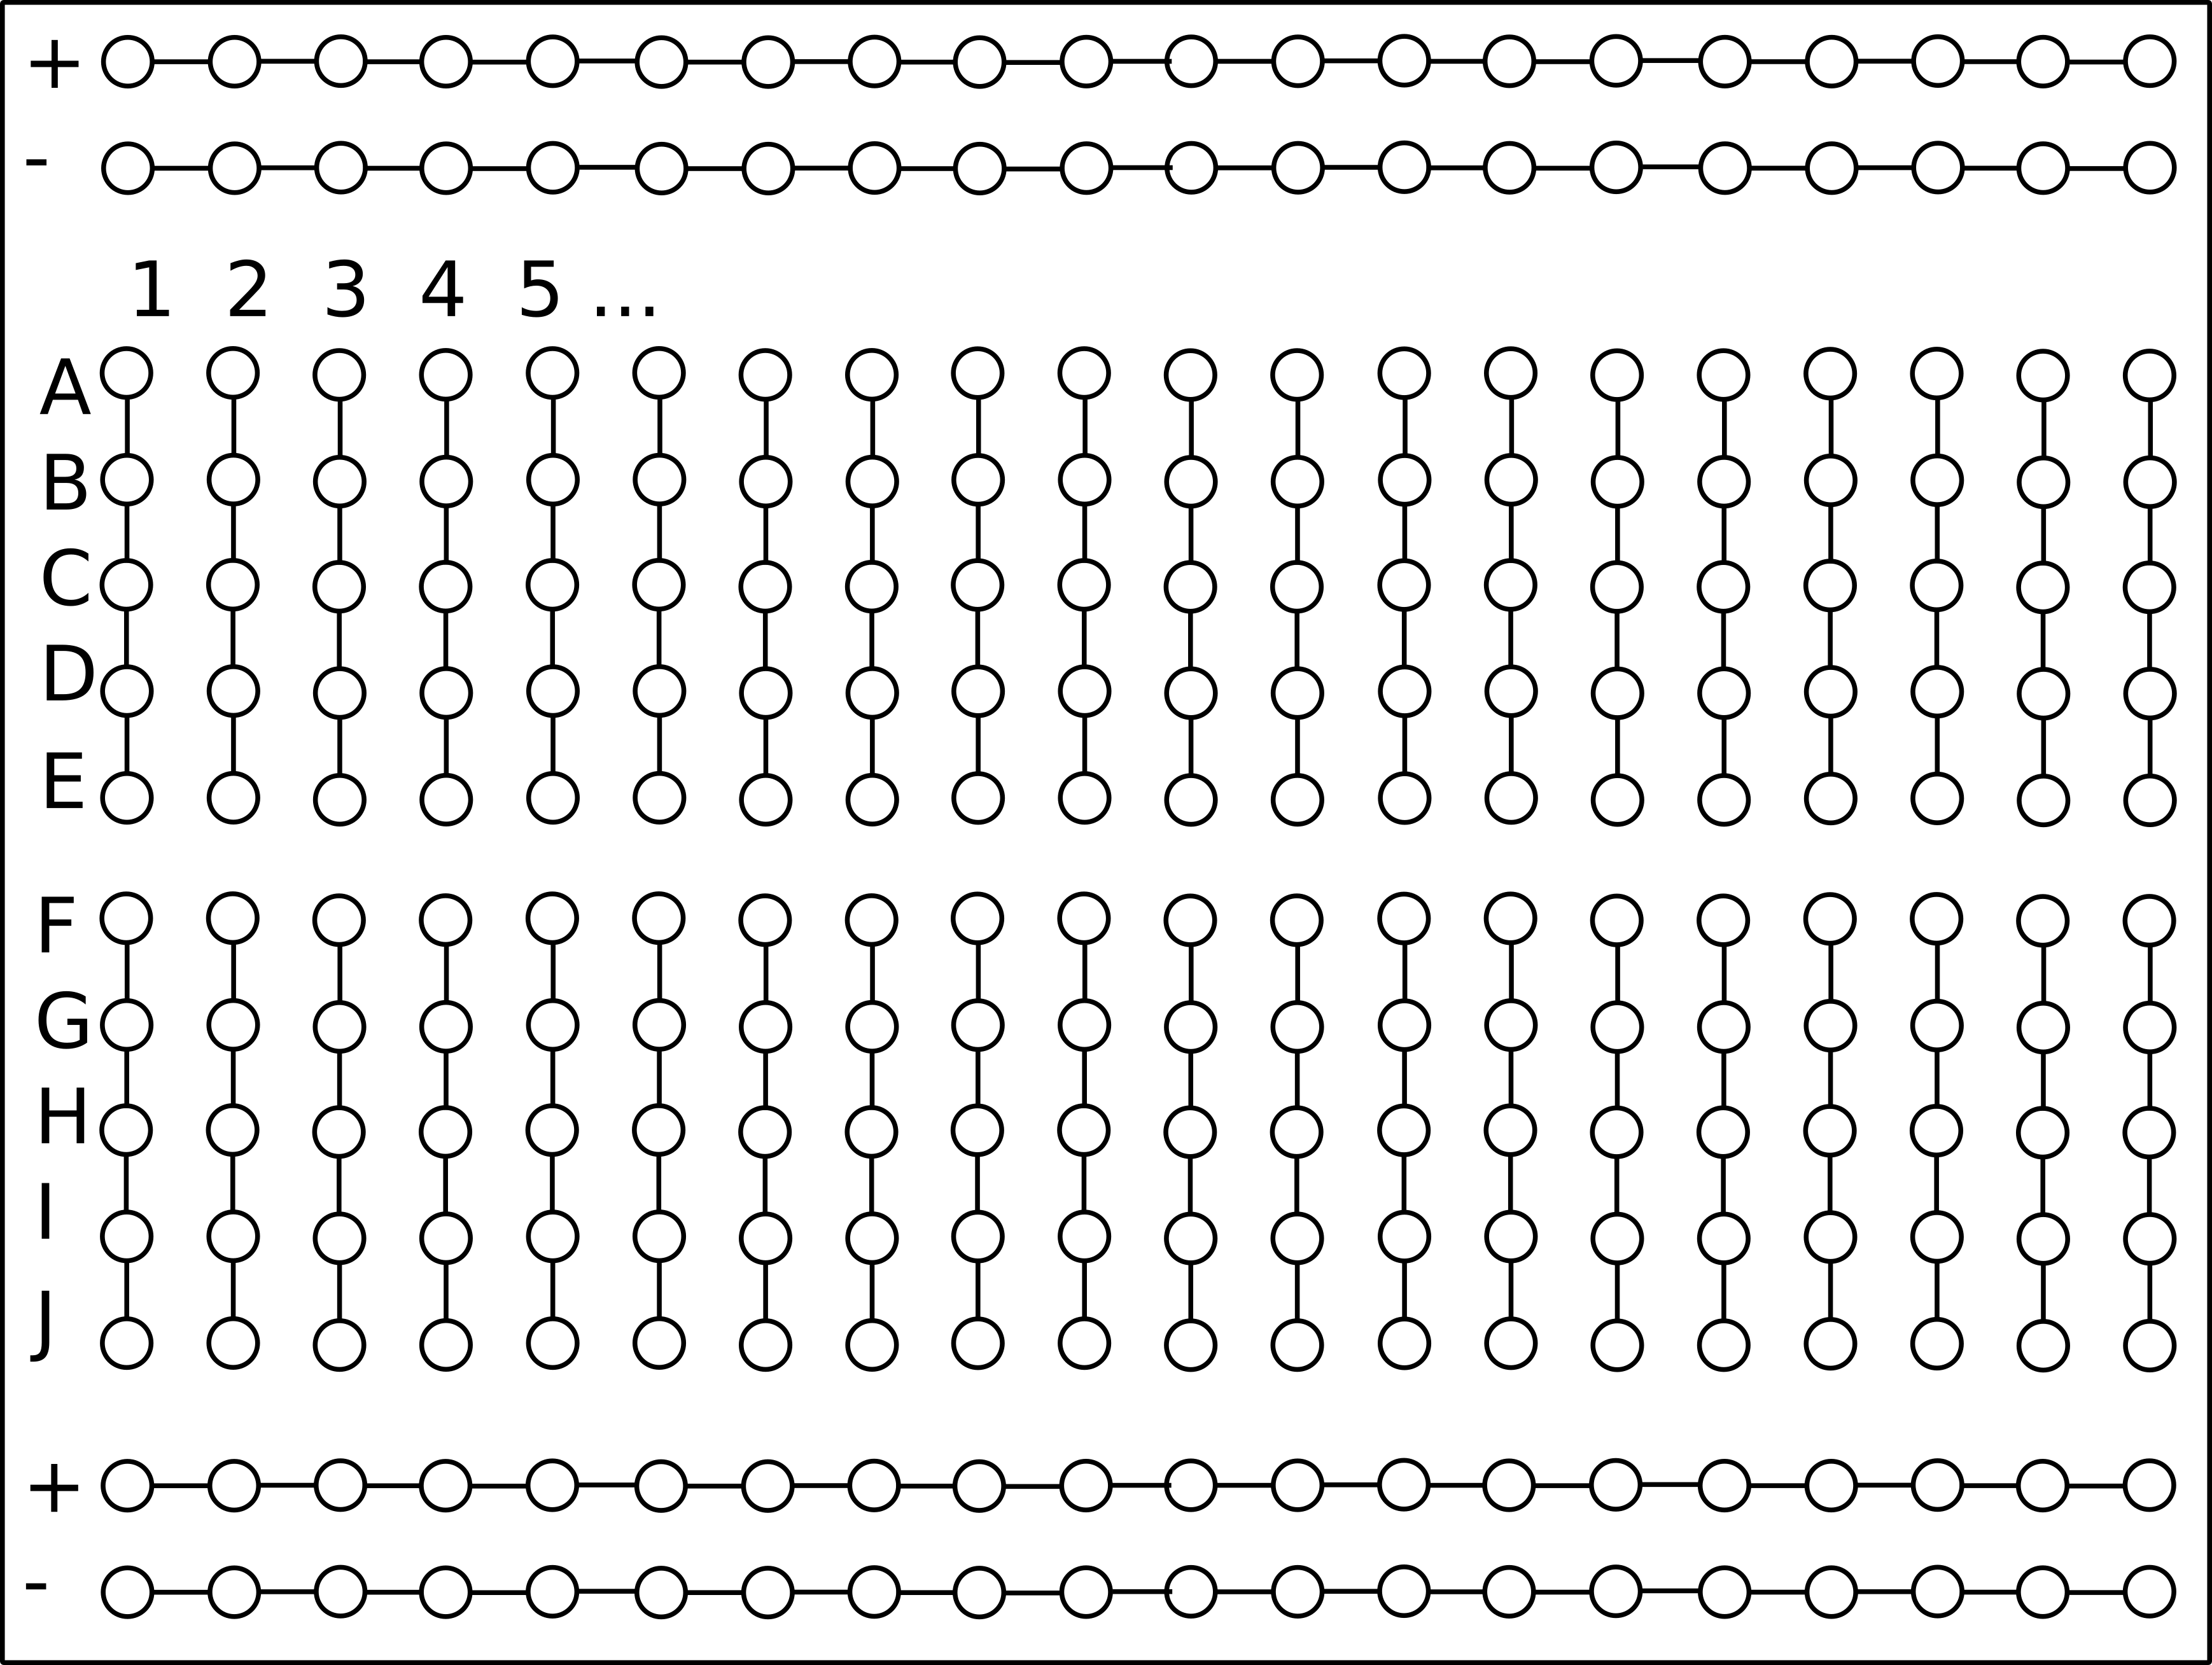
\includegraphics[scale=.050]{images/breadboard_template.png} \hspace{10mm}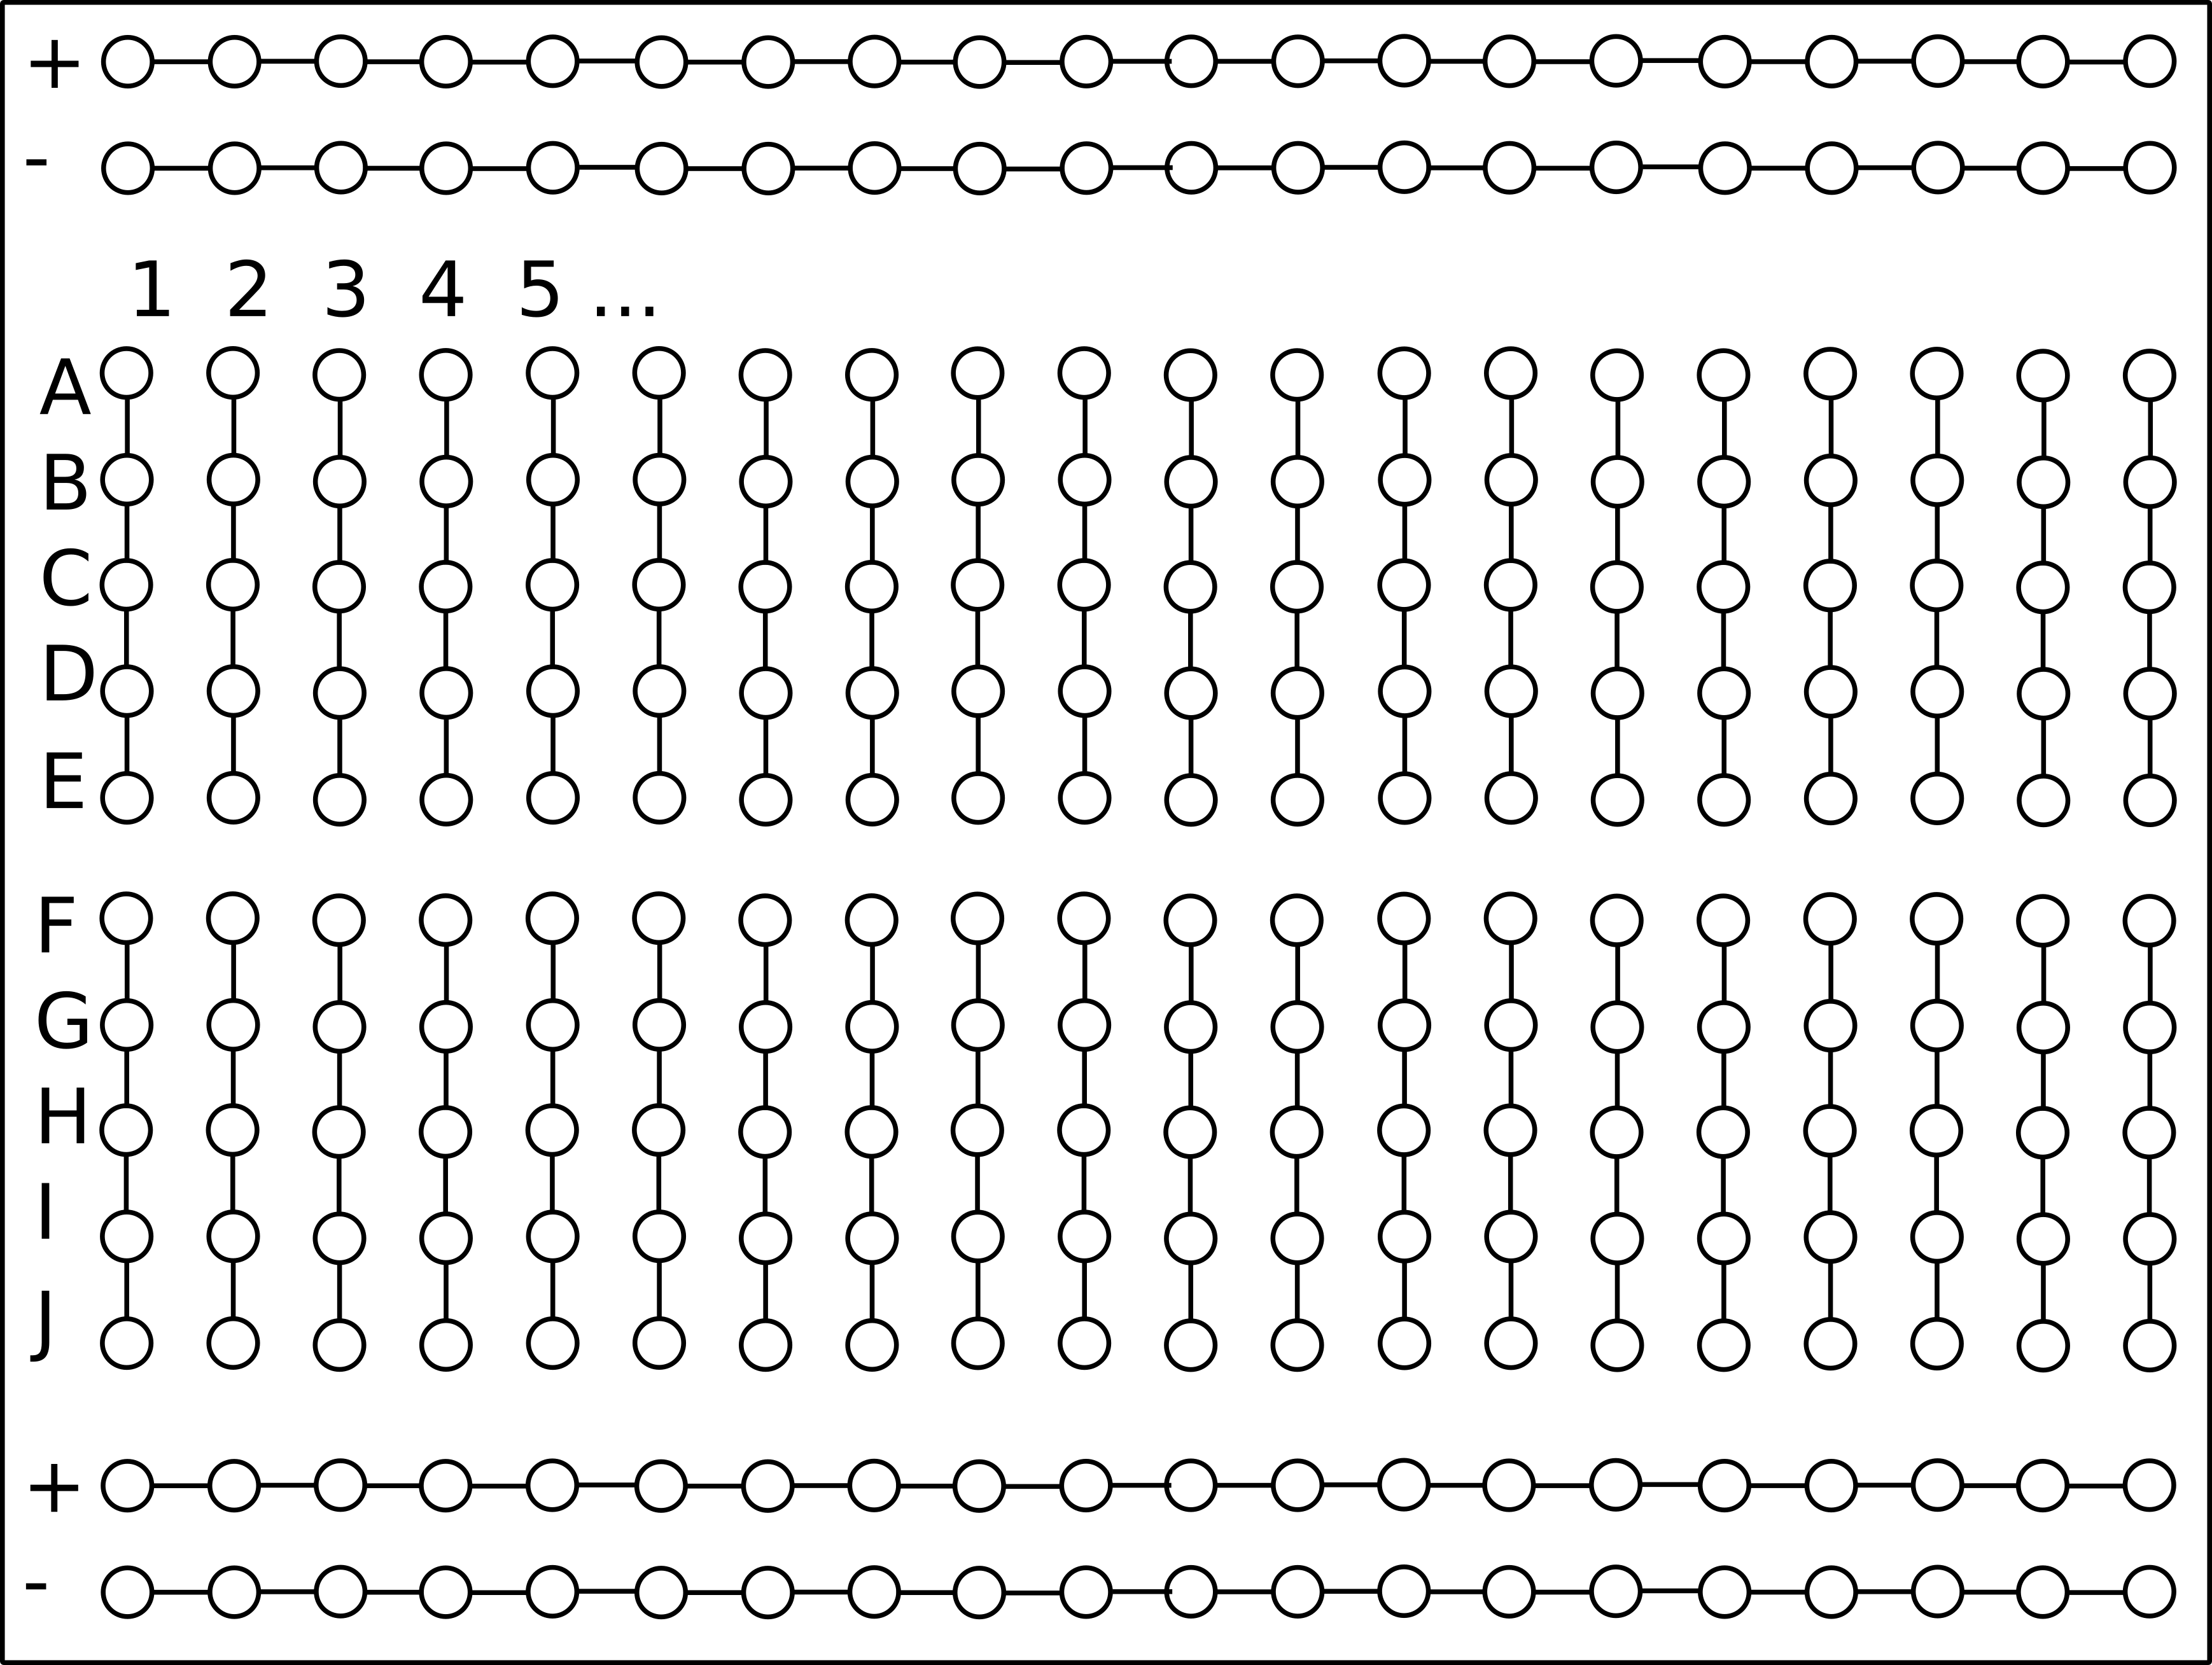
\includegraphics[scale=.050]{images/breadboard_template.png} 

			\end{frame}

			\begin{frame}
				\frametitle{\sectionIIsubsectionIVtitle}

				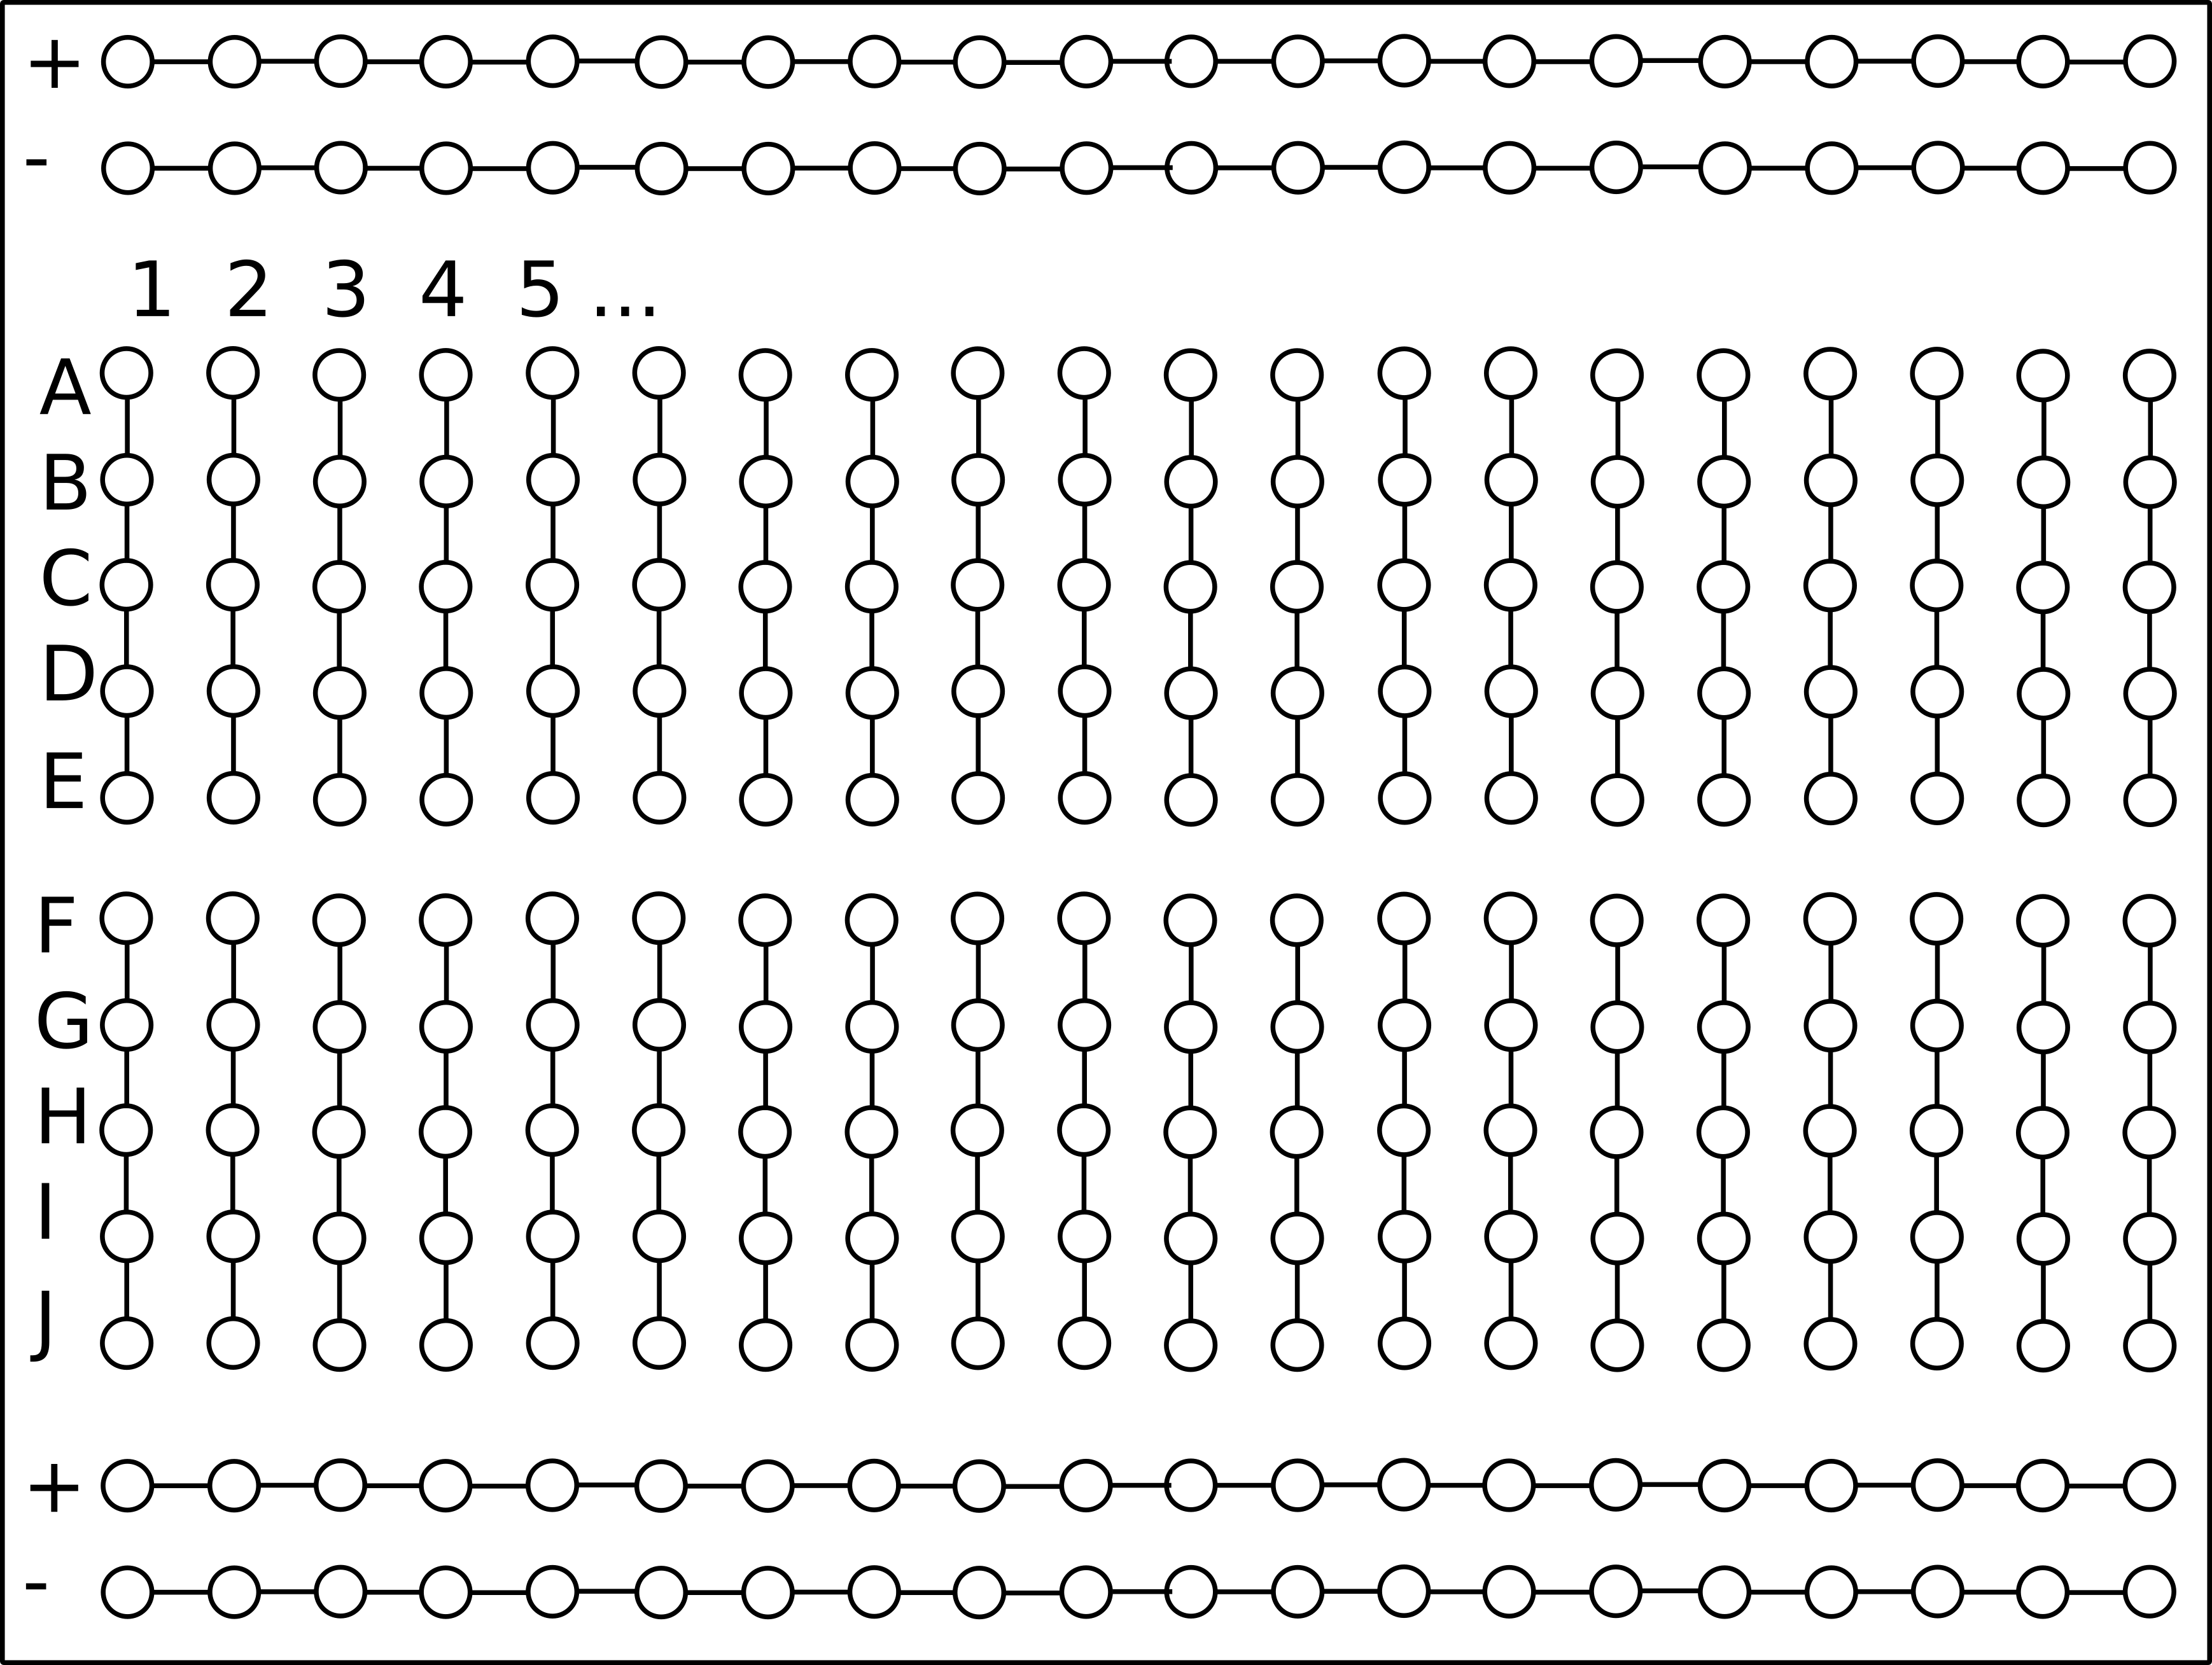
\includegraphics[scale=.050]{images/breadboard_template.png} \hspace{10mm}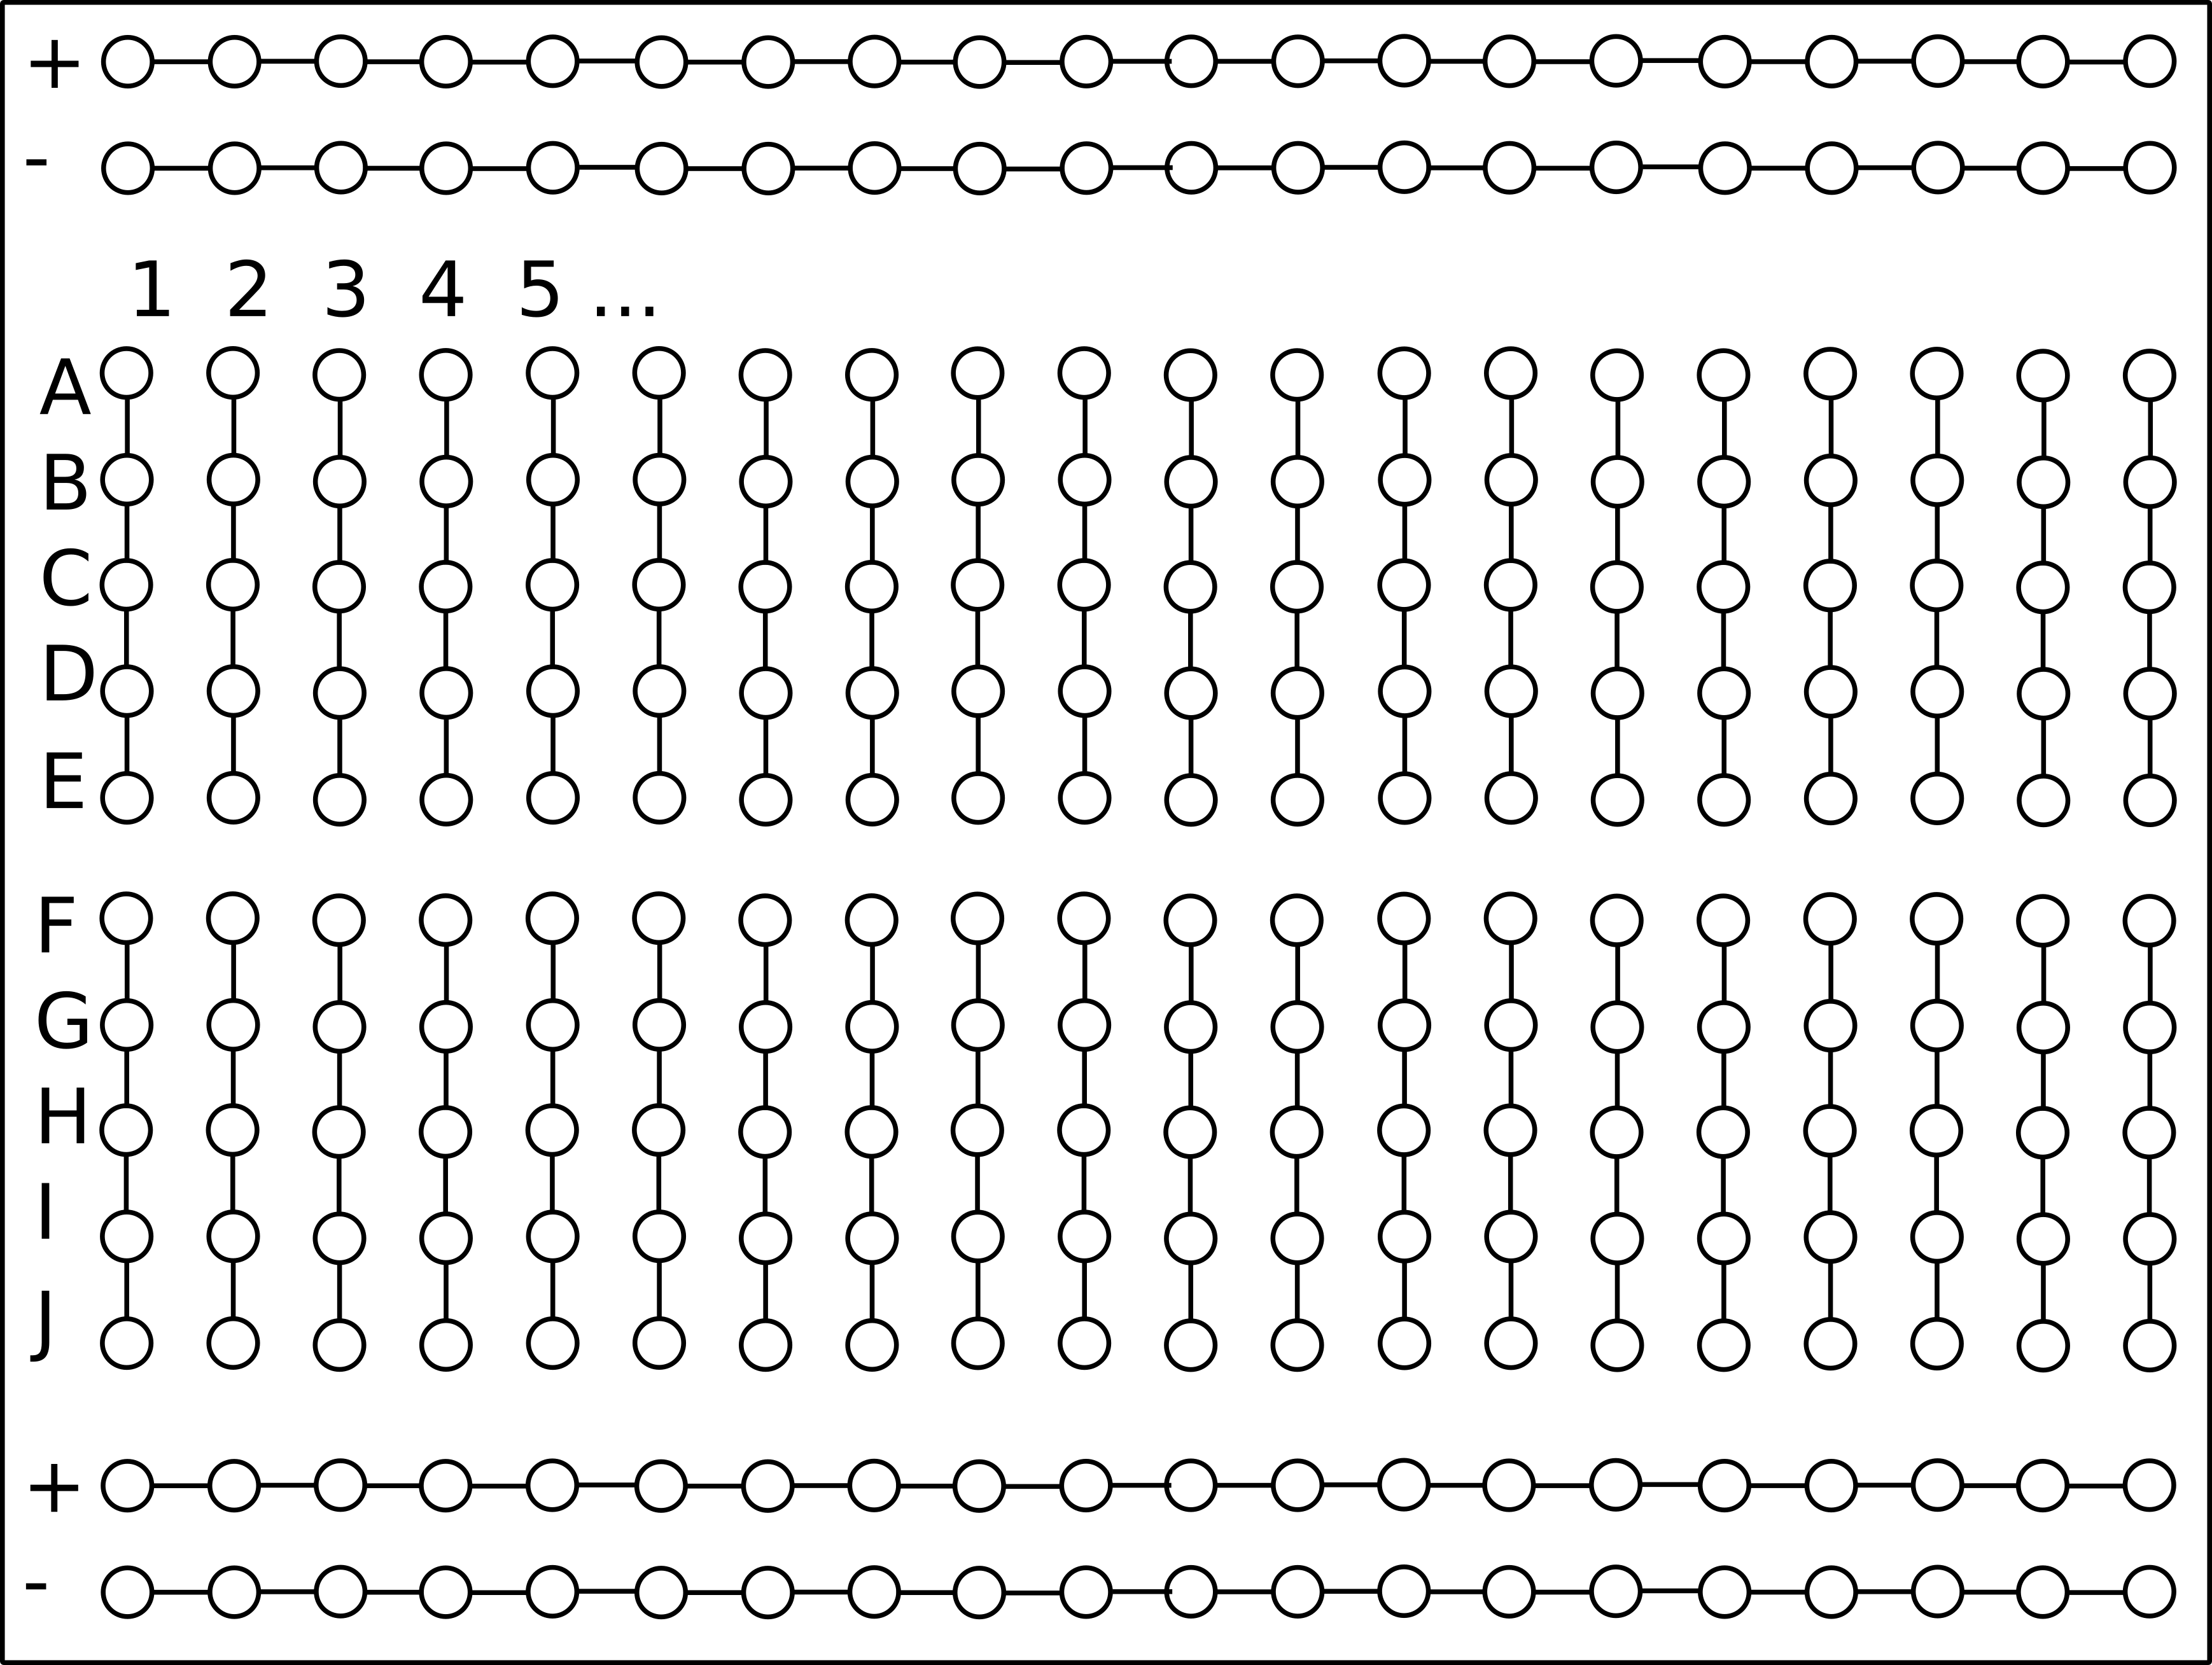
\includegraphics[scale=.050]{images/breadboard_template.png} 

			\end{frame}
		
	% Section III
	\section{\sectionIIItitle}\label{sectionIII}

		% section III Outline
		\begin{frame}
			\large \textbf{Topic 3 - \sectionIIItitle} \vspace{3mm}\\

			\begin{itemize}
				\item \hyperlink{sectionIIIsubsectionI}{\sectionIIIsubsectionItitle} \vspc %  section III subsection I
				\item \hyperlink{sectionIIIsubsectionII}{\sectionIIIsubsectionIItitle} \vspc % section III subsection II
				\item \hyperlink{sectionIIIsubsectionIII}{\sectionIIIsubsectionIIItitle} \vspc % section III subsection III
				\item \hyperlink{sectionIIIsubsectionIV}{\sectionIIIsubsectionIVtitle} \vspc % section III subsection IV
			\end{itemize}
		\end{frame}

		% section III subsection I
		\subsection{\sectionIIIsubsectionItitle}\label{sectionIIIsubsectionI}

			\begin{frame}
				\frametitle{\sectionIIIsubsectionItitle}

				
			\end{frame}

		% section III subsection II
		\subsection{\sectionIIIsubsectionIItitle}\label{sectionIIIsubsectionII}	

			\begin{frame}
				\frametitle{\sectionIIIsubsectionIItitle}

				{\tiny Text: Theory and Design of Mech. Meas.}
			\end{frame}

		% section III subsection III
		\subsection{\sectionIIIsubsectionIItitle}\label{sectionIIIsubsectionIII}

			\begin{frame}
				\frametitle{\sectionIIIsubsectionIIItitle}

			
				{\tiny Text: Theory and Design of Mech. Meas.}
			\end{frame}

		% section III subsection IV
		\subsection{\sectionIIIsubsectionIVtitle}\label{sectionIIIsubsectionIV}	

			\begin{frame}
				\frametitle{\sectionIIIsubsectionIVtitle}

			

			\end{frame}



	% Section IV
	\section{\sectionIVtitle}\label{sectionIV}



\end{document}





